\documentclass[a4paper, 11pt]{report}
\usepackage{blindtext}
\usepackage[T1]{fontenc}
\usepackage[utf8]{inputenc}
\usepackage{titlesec}
\usepackage{fancyhdr}
\usepackage{geometry}
\usepackage{fix-cm}
\usepackage[hidelinks]{hyperref}
\usepackage{graphicx}
\usepackage{multirow}
\usepackage[english]{babel}
\usepackage{xcolor}

\graphicspath{ {./images/} }

\geometry{ margin=30mm }
\counterwithin{subsection}{section}
\renewcommand\thesection{\arabic{section}.}
\renewcommand\thesubsection{\thesection\arabic{subsection}.}
\usepackage{tocloft}
\renewcommand{\cftchapleader}{\cftdotfill{\cftdotsep}}
\renewcommand{\cftsecleader}{\cftdotfill{\cftdotsep}}
\setlength{\cftsecindent}{2.2em}
\setlength{\cftsubsecindent}{4.2em}
\setlength{\cftsecnumwidth}{2em}
\setlength{\cftsubsecnumwidth}{2.5em}


\begin{document}
\titleformat{\section}
{\normalfont\fontsize{15}{0}\bfseries}{\thesection}{1em}{}
\titlespacing{\section}{0cm}{0.5cm}{0.15cm}
\titleformat{\subsection}
{\normalfont\fontsize{13}{0}\bfseries}{\thesubsection}{0.5em}{}
\titlespacing{\section}{0cm}{0.5cm}{0.15cm}

%=======================================================================================

% #########################
% IMPORTANT - Add student names here!
% e.g. \newcommand{\stud1}{LOWE, David}
\newcommand{\studA}{{RANN, Callum}}
\newcommand{\studB}{{MAI, ZIXI}}
\newcommand{\studC}{{ZHONG, QILONG}}
\newcommand{\studD}{{Li, Senhao}}
%
% IMPORTANT - Then give your SIDs
\newcommand{\sidA}{{540698143}}
\newcommand{\sidB}{{540246807}}
\newcommand{\sidC}{{540238846}}
\newcommand{\sidD}{{540220209}}
%
% IMPORTANT - And then update which major each student will focus on
\newcommand{\majA}{{Computer Science}}
\newcommand{\majB}{{Data Science}}
\newcommand{\majC}{{SW Development}}
\newcommand{\majD}{{Cyber Security}}
% #########################


\pagenumbering{Alph}
\begin{titlepage}
\begin{flushright}

\includegraphics[width=4cm]{USyd}\\[1cm]
\end{flushright}

\begin{centering}
\textbf{\huge INFO1111: Computing 1A Professionalism}\\[0.75cm]
\textbf{\huge 2024 Semester 1}\\[2cm]
\textbf{\huge Skills: Team Project Report}\\[2cm]

\textbf{\large Submission number: 3}\\[0.5cm]
\textbf{\large Github link: https://github.sydney.edu.au/INFO1111-2024/CC25-2}\\[0.75cm]
\textbf{\huge Team Members:}\\[0.75cm]

\begin{tabular}{|p{0.25\textwidth}|p{0.13\textwidth}|p{0.12\textwidth}|p{0.12\textwidth}|p{0.22\textwidth}|}
	\hline
	\multirow{2}{*}{Name} & \multirow{2}{*}{Student ID} & Target * & Target * & \multirow{2}{*}{Selected Major} \\
	 & & Foundation & Advanced & \\
	\hline
	\hline
	\raggedright{\studA} & \sidA & A & NA & \majA \\
	\hline
	\raggedright{\studB} & \sidB & A & NA & \majB \\
	\hline
	\raggedright{\studC} & \sidC & S & A & \majC \\
	\hline
	\raggedright{\studD} & \sidD & A & NA & \majD \\
	\hline
\end{tabular}
\\[0.5cm]
\end{centering}

* Use the following codes:
\begin{itemize}
\setlength\itemsep{0em}
\item NA = Not attempting in this submission
\item A = Attempting (not previously attempting)
\item AW = Attempting (achieved weak in a previous submission) 
\item AG = Attempting (achieved good in a previous submission)
\item S = Already achieved strong in a previous submission
\end{itemize}

\thispagestyle{empty}
\end{titlepage}
\pagenumbering{arabic}


%=======================================================================================

\tableofcontents

%=======================================================================================

\newpage
\section{Task 1 (Foundation): Core Skills}

Throughout your Computing degree we will help you learn a range of new skills. Once you graduate however you will need to continue to learn new languages, new tools, new applications, etc. Task 1 focuses on core technical skills (related to \LaTeX\ and Git) and the key technical skills used in different computing jobs. Each member of the team should individually complete their subsection below. You should begin by allocating to each team member a different major to focus on (i.e. one of: Computer Science; Data Science; Software Development; Cyber Security). If you have a fifth member, then your tutor will suggest a fifth topic to cover. This allocation should be specified above (see lines 37-56 in the LaTeX file).

For this section each member of your team needs to select one of the majors provided and identify 3 key technical skills that you would need to be able to work in the industry of your allocated major. You should then put these in order from most required to least required, and for each one explain why it is a key skill required for the industry of your major. You must use the skills framework for the information age ''SFIA'' to identify at least 2 out of the 3 key tech skills. (Target = $\sim$100 words per skill = $\sim$300 words total, per student).

Begin by looking at the list of skills identified within SFIA (Skills Framework for the Information Age) ~\cite{sfia}. Then select two skills from the complete list. The skills you select should be skills you believe are the most required key technical skills relevant to the major you have selected. You should explain why each skill is a key technical skill and necessary for that major.

You will need to integrate your information into the shared collaborative LaTeX document and compile the result.\\[2mm]



\textbf{OVERALL REQUIREMENTS:}

To achieve an ''OK'' rating for this task you must individually accomplish the following:
\begin{itemize}
\item Each member of your team \textbf{has been} allocated a different major (Computer Science, Data Science, Software Development, Cyber Security). 
\item Each member of your team \textbf{has identified} 3 key technical skills that you would need to be able to work in the industry of your allocated major.
	\begin{itemize}
	\item These must be in order from most required to least required.
	\item Each skill must have an explanation on why it is a key skill required for the industry of the major ($\sim$100 words per skill).
	\item At least 2 out of the 3 key tech skills must be identified from the skills framework for the information age SFIA.
	\end{itemize}
\item Github, LaTeX \& LaTeX
	\begin{itemize}
	\item Your team has created a team repository on Github for the project and put a copy of the LaTeX template, bib file, and image file into the team repository (only needs to be done by one member of your team).
	\item The information for ‘Task 1’ has been compiled into the shared collaborative LaTeX document using the template provided on Canvas with your team members sections - you have edited the LaTeX template to include your chosen major and the 3 key tech skills for the major.
	\item You have cloned the team repository to your local machine.
	\item Provide evidence that you can compile from the command line (provide screenshots of the command entered and output).
	\item Provide evidence that you can commit to your local repo (provide screenshots of the steps taken to commit to their local repo).
	\end{itemize}
\item Referencing
	\begin{itemize}
	\item You have provided in-text references (IEEE) to support your claims or where they gathered the information from.
	\item You have a reference list following the IEEE referencing guidelines.
	\item Some common things to look for to see whether your have correctly followed the referencing guide are:
		\begin{itemize}
		\item Sources are listed in alphabetical order
		\item The sources you have listed are only the sources that are present in-text.
		\item All sources seen in-text are included in the reference list.
		\item You followed the correct convention for references that don’t have author’s details or multiple sources have the same author and year of publication
		\item You have included the required information for the source type as outlined in the guide.
		\item Sources are not a list (i.e. dotpoints)
		\end{itemize}
	\end{itemize}
\end{itemize}

To achieve a ''STRONG'' rating, you must individually accomplish all of the above in addition to the following:\\
Demonstrated the following to your tutor during the tutorial:
\begin{itemize}
\item You are able to retrieve your team’s shared repo
\item You are able to make changes, recompile, commit changes, and push back to repo.
\item Note: you should also provide screen-shots of relevant actions taken to make changes, recompile etc. does not require you to provide evidence of detailing conflicts.
\end{itemize}


% =======================================================

\subsection{Skills for \majA: \studA}

Three key technical skills that are needed to work in the computer science industry:

1. Numerical analysis
Numerical analysis is the “area of mathematics and computer science that creates, analyzes, and implements algorithms for solving numerically the problems of continuous mathematics.” \cite{numan1}.  In essence, solving mathematical problems that cannot be solved analytically or symbolically, often due to their complexity or the lack of closed-form solutions. It is no doubt that the world is growing steadily more complex, resulting in “numerical analysis of increasing sophistication being needed to solve these more accurate and complex mathematical models of the world” \cite{numan2}.  

2. Computational modelling
As stated in \cite{compmodel}, proficiency in computational modeling is crucial for creating accurate representations of complex systems using mathematics, physics, and computer science. Skilled individuals can adjust variables within models to simulate various scenarios and analyze outcomes, enabling virtual experiments and hypothesis exploration. System thinking and the Turing pattern \cite{turing} emphasize the necessity of computational modelling, wherein minor adjustments to a basic formula can spawn an incomprehensibly extensive array of patterns. It is no doubt computational modeling skills accelerate the discovery and innovation process across diverse disciplines such as engineering, biology, and all other sciences. 

3. High performance computing (HPC)
HPC is ”technology that uses clusters of powerful processors that work in parallel to process massive multi-dimensional data sets” \cite{hpc2}. As \cite{hpc1} walks through, a well-known HPC solution is the supercomputer. Which displays the ability to solve more abstract problems than ever before, allowing for groundbreaking discoveries to be made.  It also majorly assists with larger data sets, which when quickly processed will allow for innovations in technologies like the Internet of Things, artificial intelligence, and 3-D imaging. Although it is extremely useful in progressing future technologies, it is not as fundamental in doing so as the previous two key techniques.

\textbf{PROOF OF GIT SKILLS}

Provide evidence that you can compile from the command line.

Compile command 1:

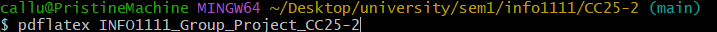
\includegraphics{Callum - compile command 1}


Output from 1 + Compile command 2:

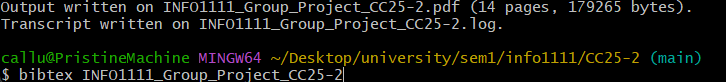
\includegraphics{Callum - compile command 2 + output from 1}


Output from 2 + Compile command 3:

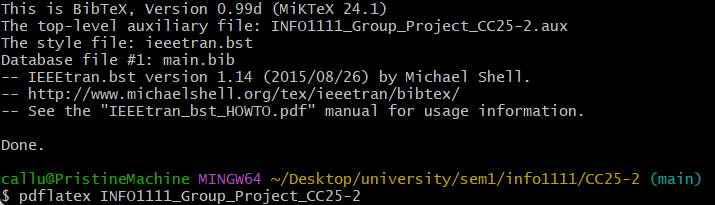
\includegraphics{Callum - compile command 3 + output from 2}


Output from 3 + Compile command 3:

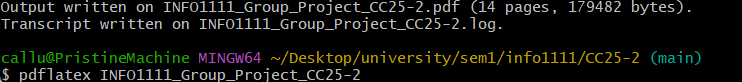
\includegraphics{Callum - compile command 4 + output from 3}


Output from 4:

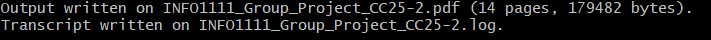
\includegraphics{Callum - output from 4}

Provide evidence that you can commit to your local repo.

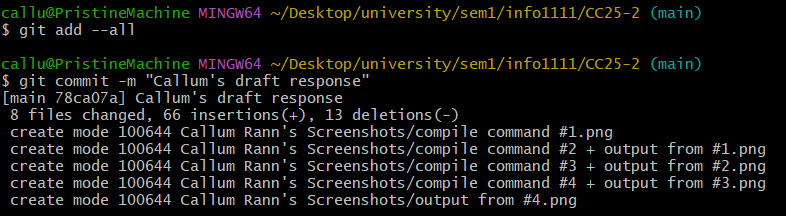
\includegraphics{Callum - local pushing guide}

\subsection{Skills for \majB: \studB}

In my opinion,the most important skills are DATS, DENG and DTAN.\\  1.Data Science: Data science serves as the fundamental knowledge base for this field\cite{van2016data}, primarily focusing on the analysis of large volumes of data characterized by high velocity and variety, encompassing numerical, symbolic, textual, auditory, and visual information. It plays a pivotal role in the entire data lifecycle, from identifying and acquiring diverse data sources to refining requirements, validating models, and evolving them over time. By uncovering intricate patterns, trends, and correlations within datasets, data science facilitates informed decision-making and propels business growth through the discovery of valuable insights. It is indispensable for making predictions, generating recommendations, and extracting deeper insights from complex data landscapes.
\\  2.Data Engineering: Data engineering includes designing, building, operationalising, securing and monitoring data pipelines and data stores, which provides the essential infrastructure and data resources that enable data science activities.\cite{birnholtz2003data} It prepares and processes data, making it accessible and usable for data scientists. Meanwhile, data science relies on data engineering support to access, analyze, and understand large-scale and heterogeneous data, enabling the discovery of valuable insights and the solution of complex problems. Thus, their relationship is symbiotic, working together to advance data-driven decision-making and business development. So DENG is a crucial part for this major.
\\  3.Data Modelling and Design: Data modeling and design involves developing models and diagrams to represent and communicate data requirements and data assets. It is essential for structuring and organizing data in a way that aligns with business requirements and analytical needs\cite{brodie1984development}, which provides the infrastructure and data structures for data science, enabling data scientists to access, understand, and analyze data effectively. Also, data science depends on the outcomes of data modelling and design to extract meaningful insights and conduct accurate analysis from structured and well-designed data. So data modelling and design is vital to this major.

\textbf{PROOF OF GIT SKILLS}

Provide evidence that you can compile from the command line.

Compile command 1 + output from 1 :

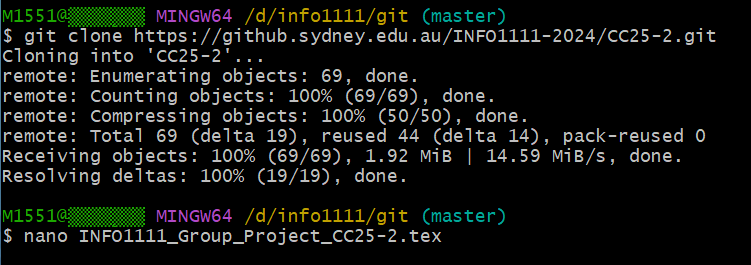
\includegraphics{ZIXI MAI clone and edit}

Compile command 2:

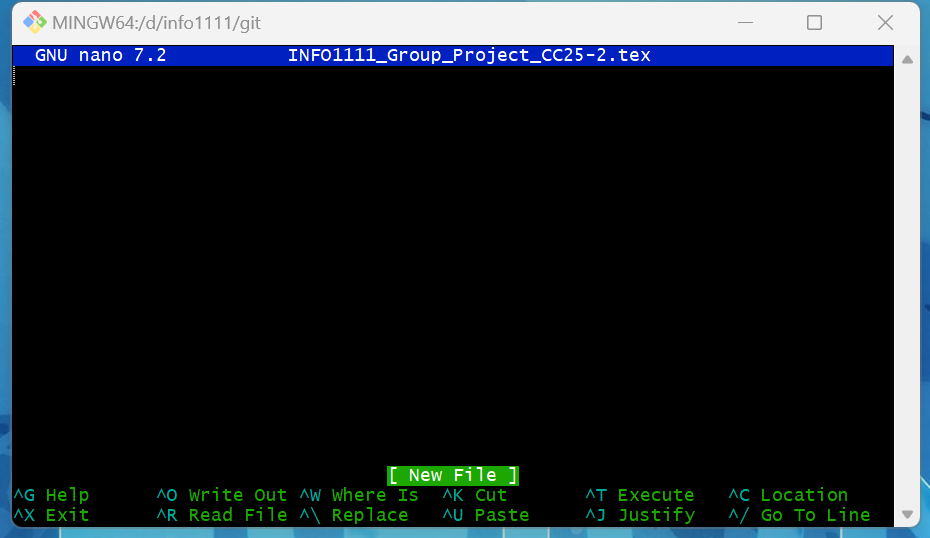
\includegraphics{ZIXI MAI edit}

Compile command 3 4 5 + output from 3 4 5:

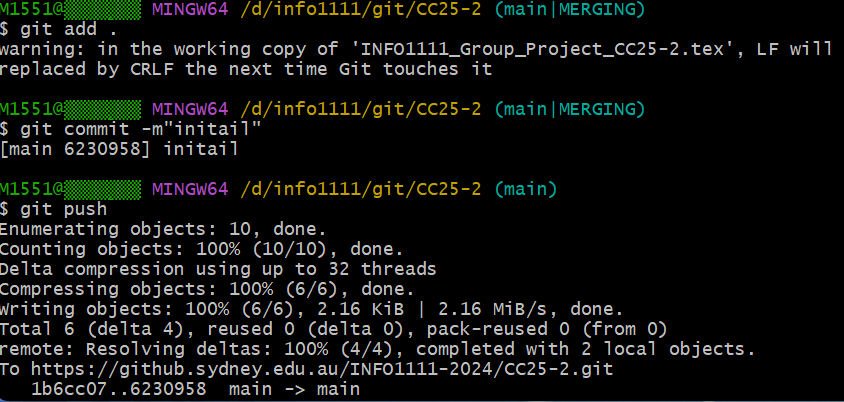
\includegraphics{ZIXI MAI push}


\subsection{Skills for \majC: \studC}

I think in descending order of importance, the three most important skills for software engineering students are Programming, Software Design and 
System Design.
\\Programming(PROG) is crucial for students in software engineering, as it is the core of building and modifying software to solve practical problems \cite{durlak1998program}. By mastering the ability of programming, not only can we use different programming languages such as Python and Java to complete our logical requirements, but we can also understand algorithms, data structures, software development cycles, and processes. Another crucial reason is that this skill can directly affect whether software design, testing, and post maintenance can be effectively implemented. Therefore, for those of us who want to make progress in the field of software development \cite{bennedsen2005revealing}, PROG is our most important skill.
\\Software Design (SWDN) is critical for software engineering students because it bridges the gap between coding skills and the creation of practical \cite{harel1990software}, efficient solutions that meet user needs. This skill directly prepares students for future roles in software engineering, making it a critical component for those seeking to stand out in a competitive field \cite{zhang2011we}. SWDN is, therefore, an indispensable skill for students aiming for strong competitiveness in the software industry.
\\System Design (DESN) is crucial for software engineering students as it enables them to design comprehensive systems that effectively integrate various software components. This skill requires students to fully understand and design the structure of the entire system, ensuring that all parts of the system work together in an orderly manner to meet the requirements \cite{boland1978process}. Mastering system design means that students can foresee how individual components will adapt to larger ecosystems, which is a key ability to develop efficient, scalable, and sustainable software solutions \cite{vasantha2012review}. This global perspective is crucial for those who wish to make significant contributions in complex software project development.

\textbf{PROOF OF GIT SKILLS}

Provide evidence that you can compile from the command line.

Compile command 1 + output from 1 + Compile command 2:

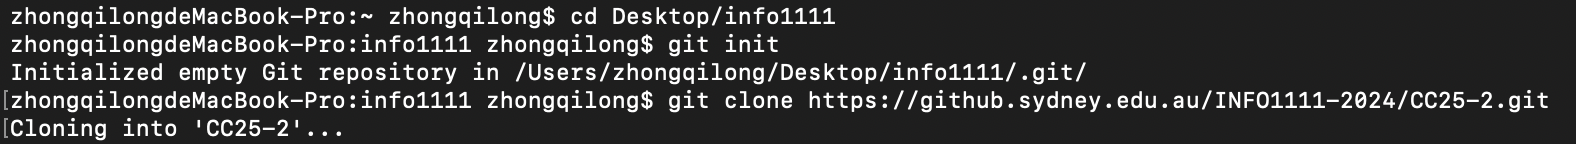
\includegraphics[scale=0.5]{Pasted Graphic}

Output 2:

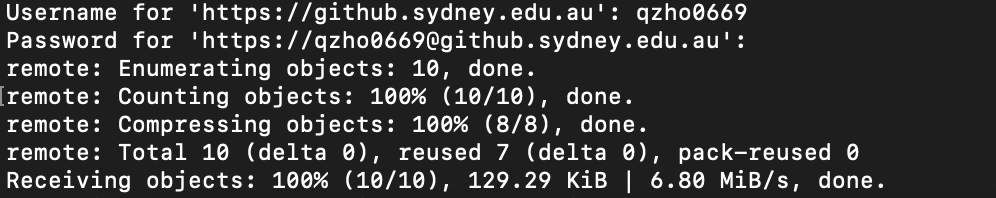
\includegraphics[scale=0.5]{Pasted Graphic 1}

Compile command 3:


\includegraphics[scale=0.5]{Pasted Graphic 2}

Output 3:

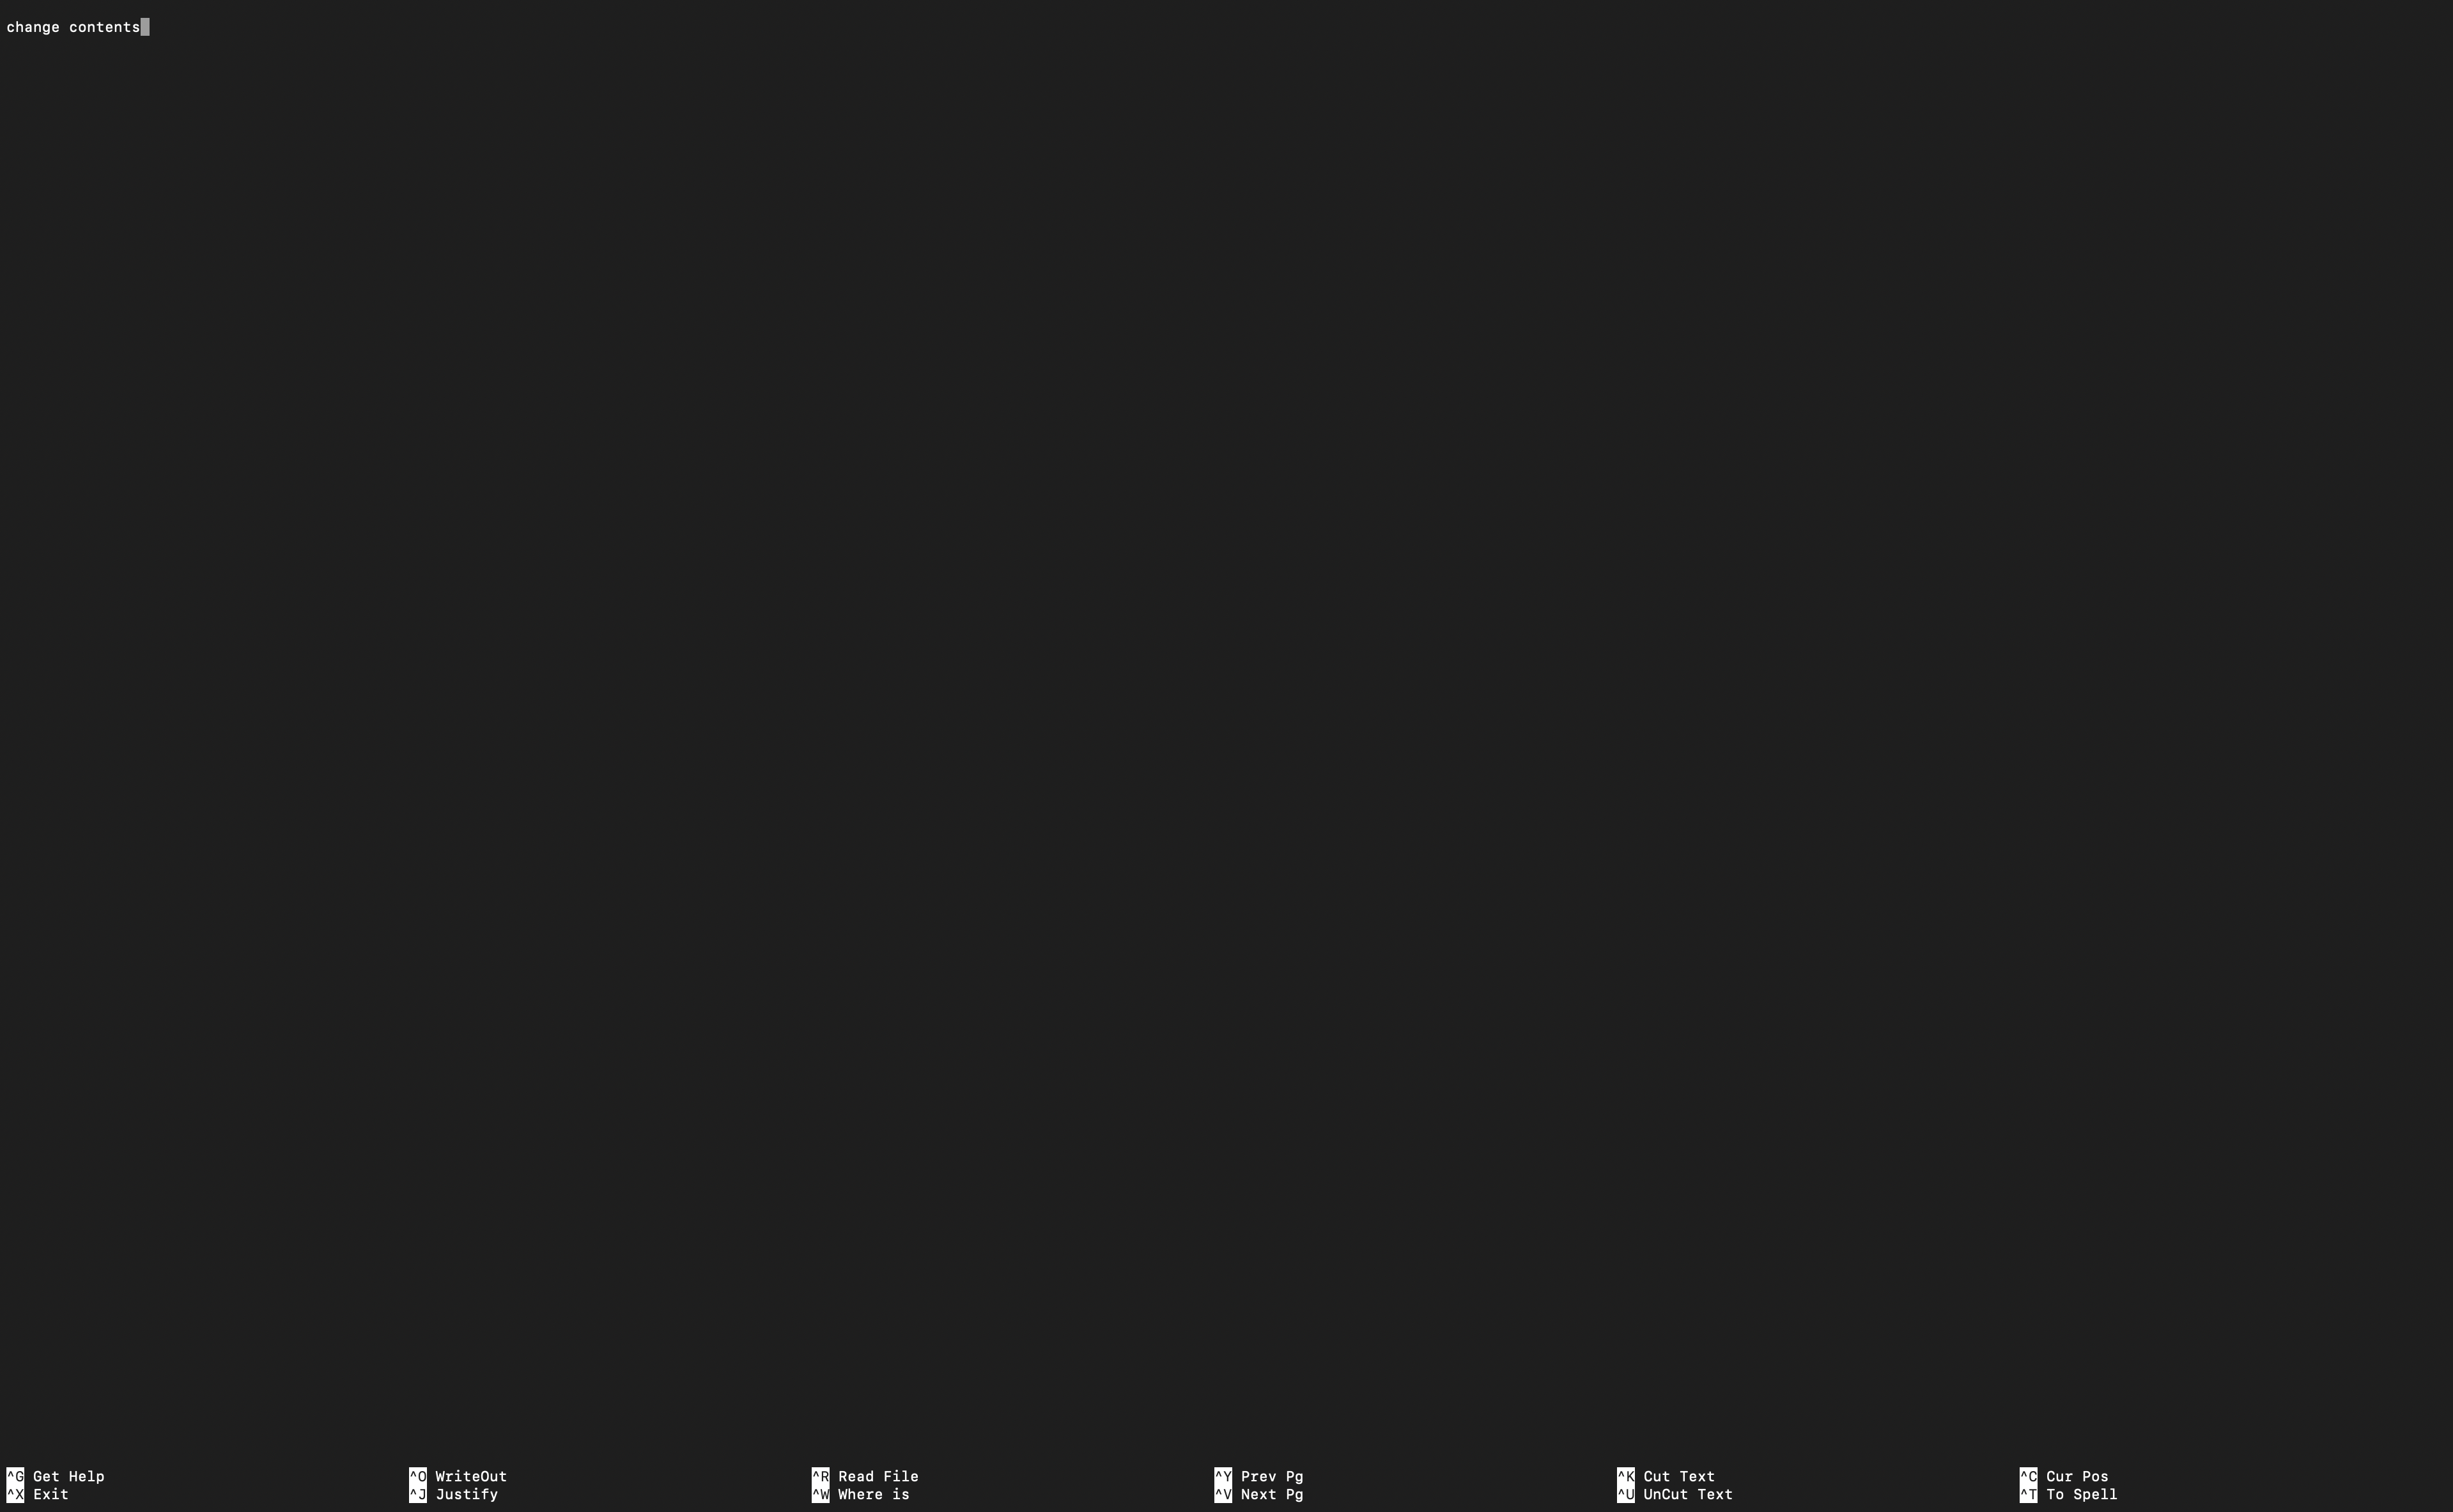
\includegraphics[scale=0.2]{Pasted Graphic 5}

Compile command 4:


\includegraphics[scale=0.25]{Pasted Graphic 6}

Compile command 5:


\includegraphics[scale=0.55]{Pasted Graphic 3}

Compile command 6 + Output 5

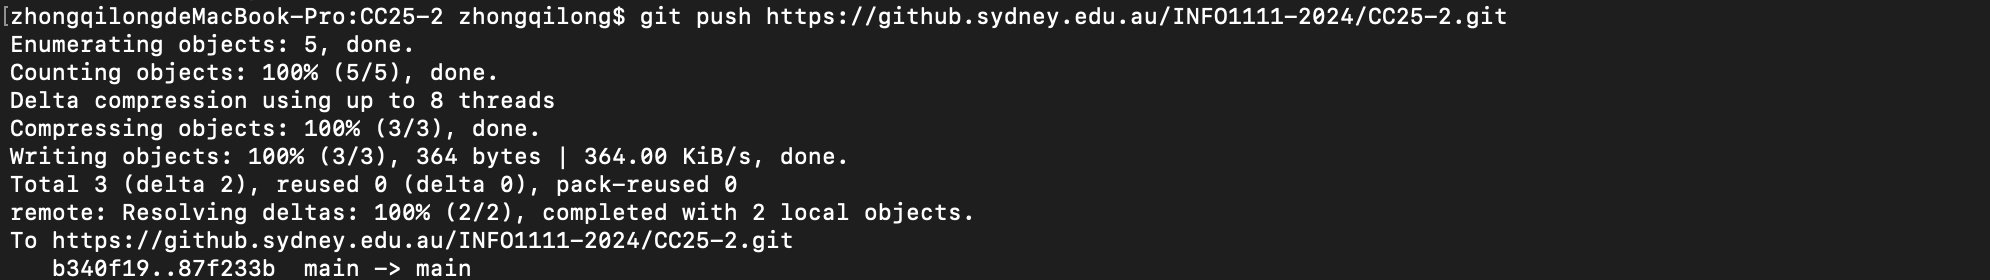
\includegraphics[scale=0.4]{Pasted Graphic 4}






\subsection{Skills for \majD: \studD}

SCTY(Information Security): It's the most important and required part for the cybersecurity industry. As stated in \cite{cyber}, It acts as a foundational skill to protect digital database from all unauthorized breaches and modifications,and addresses the core objective of cybersecurity: to protect information assets. Since the industry of cybersecurity is significant in the whole computer science, now frrequency and sophistication of cyber attacking is increasing day by day. Besides, the SCTY includes various applications of policies, technologies, and controls to safeguard related sensitive data, intellectual property, and other digital assets. Hence, this skill is really essential for every organization to guard their information privacy and enable the whole enterprise to gain customers' trust, which is bound to enhance profits and improve into a larger scale. 
\\USUP(Incident Management): Managing incidents is also crucial for efficiently and effectively ensuring security in order to avoid cyber threats or breaches. Due to its critical role in responding to and recovering from security incidents, this skill follows the extent of requirement. Through using models to macroscopically control the changes and development trends of events, the skill enables specialist in this field to protect computer effectively and easily. In addition, as stated in \cite{security}, the demand for professionals who can navigate the complexities of incident responses, including communication, analysis and recovery, is high, also owing to nowaday’s more sophisticated cyber attacks, as demonstrated in \cite{crime}. Based on such circumstance, USUP also acts as an significant skill for cybersecurity.
\\BURM(Risk Management): Though this skill is slightly less hands-on than the other two skills in direct cybersecurity activities, it’s also a key to protect the whole environment of cybersecurity. BURM involves identification, classification, assessment, organization and communication of risks followed by the application of resources to minimize, control, and monitor the impact of these risks, just like an useful assistant that helps orderly manage those risks so as not to lead to troubles, bridging the gap between cybersecurity efforts and business objectives. It ensures that security practices not only protect information assets, but also support different types of business goals, which makes it also a key strategic skill in the cybersecurity domain.

\textbf{PROOF OF GIT SKILLS}

Provide evidence that you can compile from the command line.

Compile command 1 + output from 1 + Compile command 2 + output from 2:

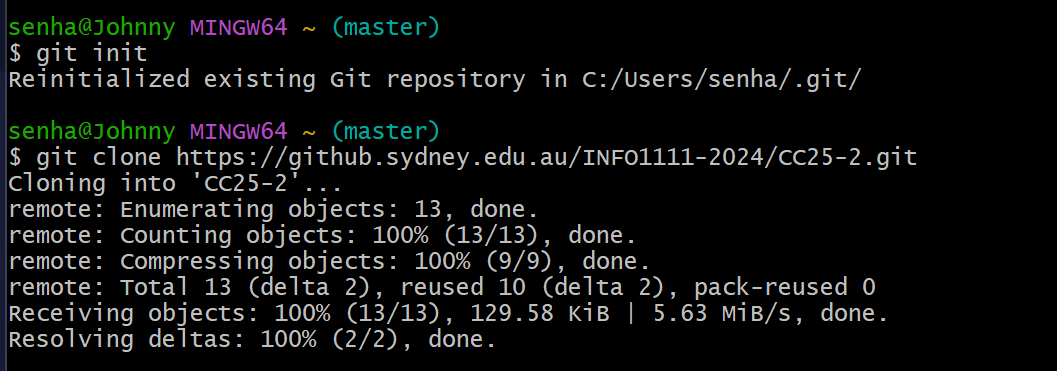
\includegraphics{graphic}

Compile command 3 + output from 3:

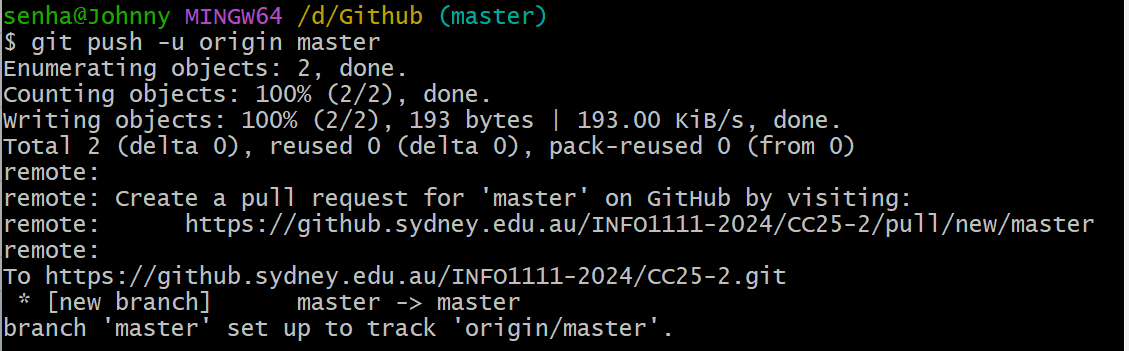
\includegraphics{graphic1}

Compile command 4 + output from 4:

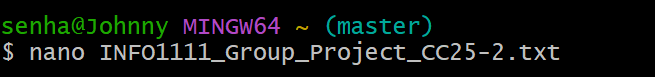
\includegraphics{graphic2}

Compile command 5 + output from 5:

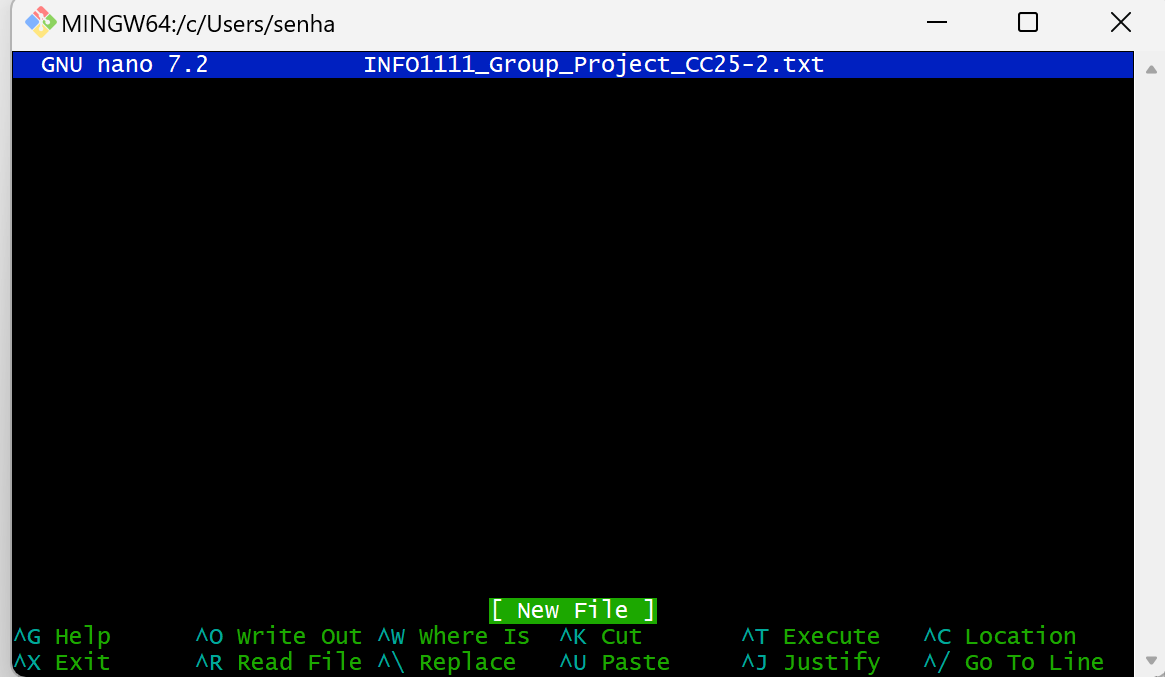
\includegraphics{graphic3}

Compile command 6 + output from 6:

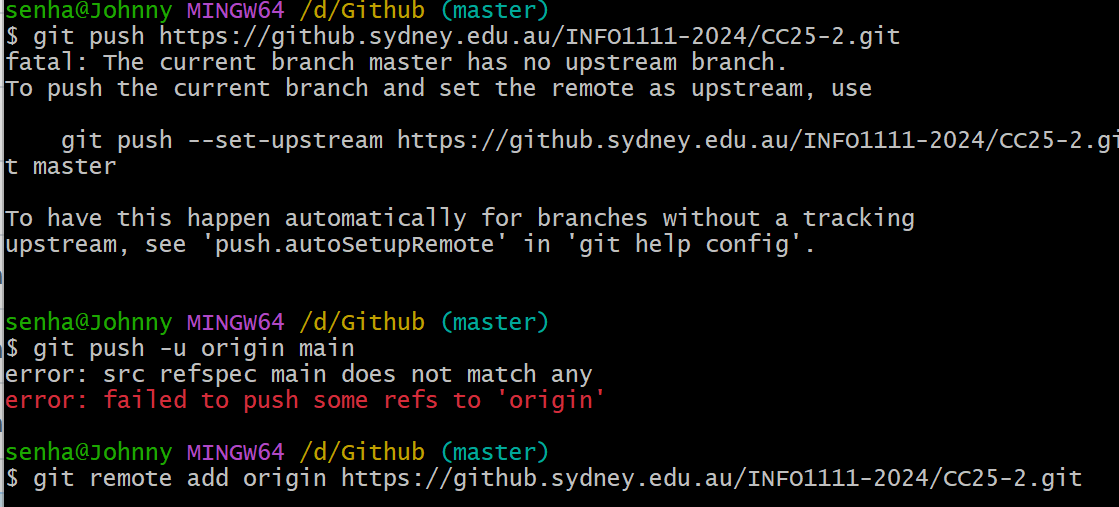
\includegraphics{graphic4}
% ========================================================

\newpage
\section{Task 2 (Advanced): Advanced Skills}

Task 2 contains two components (both required).\\[2mm]

\textbf{Component 1: Exploration of Tech Tools}

The first component focuses on exploration of relevant tech tools used within professional computing employment. All companies make use of a range of technologies and tools (often as part of a tech stack). These tools might be implementation languages; design tools; data analysis tools; collaboration technologies, etc. Each student should identify two tools that are widely used in industry, and which relate to the major you are focusing on for this project. You should then describe:

\begin{enumerate}
\item What are the two tools you have identified for your chosen major
\item The main functionality of those tools;
\item The ways in which those tools are used in the industry of your chosen major;
\item Any weaknesses or limitations of those tools.
\end{enumerate}

This task consists of two parts:

\begin{enumerate}
\item \textbf{Part A}: Generate a set of questions that you can put to ChatGPT in order to obtain answers to each of the above four questions. Using ChatGPT, then generate the answers for each of the two tools. You must include in the report below both the questions that you posed to ChatGPT, and the answers that it provided.  (100–250 words each).
\item \textbf{Part B}: For each of the four answers from Part A, assess the answer that ChatGPT provided and explain to us why you agree or disagree with the answer (100 words for each question above).
\end{enumerate}


As examples of the tools which might be selected (which you shouldn’t now use):
\begin{itemize}
\item Computer Science: Eclipse.
\item Software Development: GitHub. 
\item Cyber Security: Wireshark. 
\item Data Science: Hadoop.
\end{itemize}

Note also that no two students in the same tutorial should choose the same tools, so your tutor will maintain a list of those that have already been selected. You should therefore check this list with your tutor and then confirm your choice with your tutor prior to researching your proposed tools and spending time writing about them. (Target = $\sim$200-400 words per tool).\\[2mm]

\textbf{Component 2: Advanced LaTeX and Git Skills}

The second component of Task 2 focuses on more advanced technical skills in LaTeX and Git. The following is a list of advanced Git and LaTeX skills/features. Each student in your team that is attempting the Advanced task should select a different pair of items from each list (e.g. you might choose ''Resetting and Tags'' from the git list, and ''Cross-referencing and Custom commands'' from the LaTeX list). You then need to demonstrate actual use of each item (either through activity in Git, or through including items in this report). (Target = $\sim$100-200 words per student for each feature).

\begin{enumerate}
\item{Git}
	\begin{enumerate}
	\item Rebasing and Ignoring files 
	\item Forking and Special files 
	\item Resetting and Tags 
	\item Reverting and Automated merges 
	\item Hooks and Tags 
	\end{enumerate}
\item LaTeX 
	\begin{enumerate}
	\item Cross-referencing and Custom commands 
	\item Footnotes/margin notes and creating new environments 
	\item Floating figures and editing style sheets 
	\item Graphics and advanced mathematical equations 
	\item Macros and hyperlinks
	\end{enumerate}
\end{enumerate}
~\\[2mm]

\textbf{OVERALL REQUIREMENTS:}

To achieve an ''OK'' rating for this task you must individually accomplish the following:
\begin{itemize}
\item \textbf{Component 1 - Exploration of Tech Tools}
	\begin{itemize}
	\item Identified two tools that are widely used in industry, and which relate to the major chosen for this project.
		\begin{itemize}
		\item The two tools selected are not the same as the tools selected by other students in the tutorial. 
		\item The two tools selected are relevant to the major chosen.
		\end{itemize}
	\item Answer the following questions as instructed in 'Part A' \& 'Part B':
		\begin{itemize}
		\item What are the two tools you have identified for your chosen major
		\item 3 main functionality of each of the identified tools
		\item The ways in which those tools are used in the industry of your chosen major;
		\item 2 weaknesses or limitations of each of the tools
		\end{itemize}
	\item \textbf{Part A}: Generate a set of questions (minimum 5 questions) that can be put to ChatGPT in order to obtain answers to each of the above four questions. Using ChatGPT, then generate the answers for each of the two tools. You must include in the report below both the questions that you posed to ChatGPT, and the answers that it provided. (100 - 250 words for each question)
	\item \textbf{Part B}: For each of the four answers from Part A, assess the answer that ChatGPT provided and explain to us why they agree or disagree with the answer (100 words for each question above).
	\end{itemize}
\item \textbf{Component 2 - Advanced LaTex \& Git Skills}
	\begin{itemize}
	\item Each member of the team has selected one pair of items from each list below and demonstrate actual use of each item (i.e. a Git item and a LaTeX item).
	\item \textbf{Git}
		\begin{itemize}
		\item Rebasing and Ignoring files
		\item Forking and Special files
		\item Resetting and Tags
		\item Reverting and Automated merges
		\item Hooks and Tags
		\end{itemize}
	\item \textbf{LATEX}
		\begin{itemize}
		\item Cross-referencing and Custom commands
		\item Footnotes/margin notes and creating new environments
		\item Floating figures and editing style sheets
		\item Graphics and advanced mathematical equations
		\item Macros and hyperlinks
		\end{itemize}
	\item This means no two members of the team have not chosen the same item from either of the lists above.
	\item You have demonstrated the use of your selected items either through activity in Git, or through including items in this report.
	\item This means for Git items:
		\begin{itemize}
		\item You have added your tutor to your git repository and when they view it they are able to see your activity that demonstrates the use of your selected items (e.g. forks, hooks, tags, merges etc.).
		\item You have included screenshots and annotations (where necessary) in your report and provided an explanation of $\sim$100 words of your use of advanced Git features.
		\end{itemize}
	\item and for LaTeX items:
		\begin{itemize}
		\item You have included items you have chosen in your LaTeX report document submission and the tutor is able to clearly see it (e.g. the pdf document written in LaTeX has hyperlinks, macros, cross referencing etc. included in it).
		\item You have included screenshots and annotations (where necessary) in your report and provided an explanation of $\sim$100 words of your use of advanced LaTeX features.
		\end{itemize}
	\end{itemize}
\item Referencing
	\begin {itemize}
	\item You have provided in-text references (IEEE) to support your claims or where they gathered the information from.
	\item You have a reference list following the IEEE referencing guidelines.
		\begin{itemize}
		\item Some common things to look for to see whether your have correctly followed the referencing guide are:
		\item Sources are listed in alphabetical order
		\item The sources you have listed are only the sources that are present in-text.
		\item All sources seen in-text are included in the reference list.
		\item You followed the correct convention for references that don’t have author’s details or multiple sources have the same author and year of publication
		\item You have included the required information for the source type as outlined in the guide.
		\item Sources are not a list (i.e. dotpoints)
		\end{itemize}
	\end{itemize}
\end{itemize}

To achieve a ''STRONG'' rating you must accomplish all of the above in addition to the following:
\begin{itemize}
\item The answers provided to the 4 questions (component 1b) use ChatGPT and independent research and analysis is excellent, showing a deep understanding of industry.
\item You have used advanced Git features such as branching when demonstrating the items you selected (component 2a).
\end{itemize}



% ========================================================

\subsection{Tools and Skills for \majA: \studA}

\subsubsection{Part A: Exploration of tech tools}

\textbf{\large{Tool Identification}}

The two tools identified for the Computer Science major was taken from industry guest presentation in week 7. From here I chose tools that offered functions I was not familiar with, in this case Docker’s containerisation, and Poetry’s package management.  I was able to confirm these were widely used in industry by searching for the reccommended tools for these functions and these two popping up on multiple occassions \cite{topcontainers}, \cite{pythonpackagemanagers}. 

\vspace{\baselineskip}
\textbf{\large{Tool 1 Questions - Docker}}

\textbf{Question 1: What is the main functionality of thecomputer science tool Docker, in 250 words or less?}  

Docker is a powerful tool used in computer science primarily for containerization. It allows developers to package their applications and dependencies into standardized units called containers, which can then be easily deployed across different computing environments, from local machines to cloud servers. 

The main functionality of Docker revolves around creating, managing, and deploying these containers. It provides a lightweight runtime environment that encapsulates the application and all its dependencies, ensuring consistency and reliability across various platforms. 

With Docker, developers can build their applications in a consistent environment, eliminating the "it works on my machine" problem often encountered in software development. Containers created with Docker are portable and can run seamlessly on any system that supports Docker, regardless of the underlying infrastructure. 

Docker also streamlines the development workflow by enabling rapid deployment and scaling of applications. Developers can quickly spin up containers, test their applications, and deploy updates without worrying about compatibility issues or configuration differences between environments. 

Furthermore, Docker facilitates microservices architecture, allowing developers to break down complex applications into smaller, manageable components deployed as separate containers. This modular approach enhances scalability, flexibility, and maintainability of software systems. 

Overall, Docker revolutionizes the way applications are developed, shipped, and run by providing a standardized and efficient containerization solution that simplifies deployment and management processes while promoting consistency and reproducibility in software development. 

 \vspace{\baselineskip}
\textbf{Question 2: How is Docker used in the computer science industry, in 250 words or less?}

In the computer science industry, Docker is extensively used across various stages of the software development lifecycle. Initially, developers utilize Docker to create isolated development environments, ensuring consistency between different team members' setups and reducing "it works on my machine" issues. They package their applications and dependencies into Docker containers, which can be easily shared and replicated across development, testing, and production environments. 

During testing, Docker facilitates continuous integration and continuous deployment (CI/CD) pipelines by automating the process of building, testing, and deploying applications. Integration with tools like Jenkins or GitLab CI allows for seamless integration of Docker containers into the testing workflow, enabling faster and more reliable delivery of software updates. 

In production environments, Docker provides a lightweight and efficient platform for deploying and managing applications at scale. It enables organizations to adopt microservices architecture, breaking down monolithic applications into smaller, decoupled services deployed as independent containers. This approach improves scalability, fault isolation, and resource utilization, allowing for easier maintenance and updates. 

Moreover, Docker plays a crucial role in cloud computing, enabling cloud-native development and deployment practices. Platforms like Kubernetes leverage Docker containers to orchestrate and manage complex distributed systems, automating tasks such as scaling, load balancing, and service discovery. 

Overall, Docker revolutionizes software development and deployment practices in the computer science industry by providing a standardized and efficient containerization solution that improves consistency, scalability, and agility across the software development lifecycle. 

\vspace{\baselineskip}
\textbf{Question 3: Does Docker have any weaknesses or limitations, in 250 words or less?}

Yes, Docker, like any technology, has its share of weaknesses and limitations. These include: 

Performance Overhead: Docker introduces a slight performance overhead due to the additional layer of abstraction it adds. While usually minimal, this overhead can impact resource utilization, especially in high-performance computing environments. 

Security Concerns: Docker containers share the same kernel as the host system, which poses security risks. Vulnerabilities in the kernel or misconfigurations could potentially allow containerized applications to access host resources, leading to security breaches. 

Persistence and State Management: Docker containers are typically designed to be stateless and ephemeral. Managing persistent data and stateful applications within Docker containers can be challenging and may require additional configurations or external storage solutions. 

Learning Curve: Docker introduces new concepts and terminologies, which may have a learning curve for users unfamiliar with containerization. Understanding how to create efficient Dockerfiles, manage images, and orchestrate containers with tools like Docker Compose or Kubernetes requires time and effort. 

Compatibility Issues: Docker dependencies on specific versions of Docker Engine and container runtimes can lead to compatibility issues. Ensuring compatibility between different versions of Docker and containerized applications can be a concern, particularly in large-scale deployments with diverse environments. 

Despite these limitations, Docker remains a powerful tool for containerization, offering significant benefits in terms of portability, scalability, and efficiency for modern software development and deployment. 

\vspace{\baselineskip}
\vspace{\baselineskip}
\textbf{\large{Tool 2 Questions - Poetry}}
  
\textbf{Question 1: What is the main functionality of the computer science tool Poetry, in 250 words or less?}

Poetry is a tool primarily used for managing Python dependencies and virtual environments. It simplifies the process of dependency management by providing a robust and consistent approach. With Poetry, developers can define project dependencies and their versions in a pyproject.toml file, similar to other modern package managers like npm or pipenv. 

One of its main features is dependency resolution, which ensures that all dependencies are compatible with each other and with the Python version specified for the project. Poetry also creates and manages isolated virtual environments for each project, preventing conflicts between dependencies across different projects. 

Furthermore, Poetry facilitates package publishing to PyPI, making it easy for developers to share their Python projects with the community. It automates tasks such as building and publishing packages, saving developers time and effort. 

Overall, Poetry streamlines the Python development workflow by providing a comprehensive solution for dependency management, virtual environment creation, and package publishing. Its user-friendly interface and powerful features make it a popular choice among Python developers for managing project dependencies and ensuring project stability and compatibility. 

\textbf{Question 2: How is Poetry used in the computer science industry, in 250 words or less?} 

In the computer science industry, Poetry is widely used to streamline Python development workflows, particularly in projects of varying scales and complexities. Its popularity stems from several key factors. 

Firstly, Poetry simplifies dependency management by allowing developers to define project dependencies in a single pyproject.toml file. This eliminates the need for complex requirements.txt files or manual dependency tracking, reducing errors and ensuring consistency across development environments. 

Secondly, Poetry automates the creation and management of virtual environments, which are isolated environments where project dependencies can be installed without affecting system-wide Python installations. This isolation prevents conflicts between dependencies and ensures project stability. 

Thirdly, Poetry's dependency resolution algorithm ensures that all dependencies are compatible with each other and with the specified Python version. This helps prevent dependency hell and ensures that projects can be easily reproduced on different systems. 

Additionally, Poetry provides tools for packaging and publishing Python projects to platforms like PyPI, simplifying the process of sharing code with the wider community or within an organization. This makes it easier for developers to collaborate and contribute to open-source projects. 

Overall, Poetry has become an essential tool in the computer science industry for managing Python projects efficiently and reliably. Its user-friendly interface, robust features, and focus on best practices make it a go-to choice for developers looking to streamline their development workflows and ensure project success. 

 \textbf{Question 3: Does Poetry have any weaknesses or limitations, in 250 words or less?}

While Poetry offers numerous benefits for managing Python projects, it's not without its limitations and potential drawbacks. 

One limitation is that Poetry's integration with certain development environments or continuous integration (CI) systems may not be as seamless as with other tools. While it has improved compatibility over time, some setups may require additional configuration or workarounds to fully integrate Poetry into the development workflow. 

Another consideration is that Poetry is still relatively young compared to more established tools like pipenv or traditional requirements.txt files. As a result, it may lack some features or integrations that users have come to expect from more mature tools. However, the Poetry community is actively working to address these limitations and improve the tool's functionality. 

Furthermore, while Poetry excels at managing Python dependencies, it may not be the best choice for projects with complex multi-language dependencies or specialized requirements outside of Python development. 

Additionally, there may be a learning curve for developers who are accustomed to other dependency management tools or workflows. Transitioning to Poetry may require time and effort to become familiar with its unique features and conventions. 

Despite these limitations, Poetry continues to evolve and gain traction in the Python community due to its focus on simplicity, reliability, and modern best practices. As with any tool, it's essential to evaluate Poetry's strengths and weaknesses in the context of your specific project requirements and development workflow. 

\subsubsection{Part B: Analysis}

\textbf{\large{Tool 1 Response Evaluation - Docker}}

\textbf{Functionality of Docker:} \\
\noindent ChatGPT's response effectively captures Docker's primary functionality, closely echoing the content provided in \cite{dockeroverview}. Docker is described as a platform for developing, shipping, and running applications, "Docker enables you to separate your applications from your infrastructure so you can deliver software quickly". This aligns with ChatGPT's explanation of Docker's role in containerization, which allows developers to package applications and dependencies into standardized units called containers. Therefore, ChatGPT's response provides an accurate summary of Docker's main functionality.

\textbf{Usage of Docker in the computer science industry:} \\
\noindent ChatGPT's response accurately outlines Docker's usage across various stages of the software development lifecycle, which closely mirrors the content provided in \cite{dockeroverview}. The source emphasizes Docker's significance in continuous integration and continuous delivery workflows, stating that "Containers are great for continuous integration and continuous delivery (CI/CD) workflows". Similarly, ChatGPT highlights Docker's role in facilitating CI/CD pipelines during testing and deployment phases. Therefore, ChatGPT's response aligns well with the provided source, effectively summarizing Docker's usage in the computer science industry.

\textbf{Weaknesses or limitations of Docker: } \\
\noindent ChatGPT's response identifies several weaknesses and limitations of Docker, which are consistent with the drawbacks outlined in \cite{dockerlimits}. The source mentions security risks associated with Docker containers, stating that "Docker containers are not completely isolated from the host system". Similarly, ChatGPT mentions security concerns as one of Docker's limitations. Furthermore, the source discusses the complexity of Docker adoption, stating that "Docker can be complex to learn and use", which aligns with ChatGPT's point about Docker's learning curve. Therefore, ChatGPT's response provides a balanced assessment of Docker's strengths and weaknesses, effectively summarizing key points from the provided source.

In conclusion, ChatGPT's responses accurately summarize Docker's functionality, usage, and limitations, aligning closely with the information provided in the sources. 

\vspace{\baselineskip}\\
\noindent \textbf{\large{Tool 2 Response Evaluation - Poetry}}

\textbf{Functionality of Poetry:} \\
\noindent ChatGPT's response accurately portrays Poetry as a tool for managing Python dependencies and virtual environments, simplifying dependency management with a consistent approach. This aligns with the functionality described "Poetry is a tool for dependency management and packaging in Python. It allows you to declare the libraries your project depends on and it will manage (install/update) them for you."  \cite{poetryoverview}.

Additionally, Poetry offers features like a lockfile to ensure repeatable installs and project distribution capabilities. ChatGPT's response effectively captures Poetry's primary functionality, as described in the source. 

\textbf{Usage of Poetry in the Computer Science Industry:} \\
\noindent ChatGPT describes Poetry's widespread adoption in the computer science industry for streamlining Python development workflows. While not directly quoting \cite{poetrylimits}, which mentions considering Poetry for managing Python applications, the response captures the essence of the source by emphasizing Poetry's role in improving dependency management in Python projects. 

\textbf{Weaknesses or Limitations of Poetry:} \\
\noindent ChatGPT acknowledges Poetry's limitations, such as integration challenges and potential drawbacks. These limitations are consistent with the experiences shared in \cite{poetrylimits}, where users mention issues with extra dependencies and build-time concerns when adopting Poetry for dependency management. One user expresses concerns about Poetry's impact on their workflow: 

"Easily the biggest pain-point of having moved to, and now wanting to move away from, poetry is that you now have an extra build-time and / or runtime dependency you have to install on the system prior to installing your dependencies." 

This quote highlights the practical challenges users may encounter when transitioning to Poetry, supporting ChatGPT's assertion regarding Poetry's limitations. 

Overall, ChatGPT's responses effectively integrate information from the provided sources, providing a comprehensive evaluation of Poetry's functionality, usage, and limitations. The inclusion of quotes strengthens the evaluation by directly referencing user experiences and descriptions of Poetry's functionality from the sources. Therefore, ChatGPT's responses can be considered accurate assessments of Poetry based on the given sources. 

\subsubsection{Technical Skills (LaTeX and Git)}

 \textbf{\large{Git Skill: Rebasing and Ignoring Files}}

\vspace{\baselineskip}
\textbf{Rebasing:}

Rebasing provides an alternative to merging, rather than presenting the joining of branches as a single merge commit, it sends the new branches one by one, allowing for a more linear history and easier conflict resolution.  

Here is an example: 

\begin{itemize}
\item Original logs of master branch 
\end{itemize}
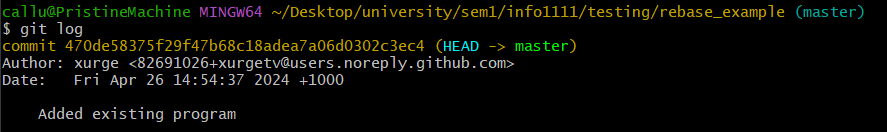
\includegraphics[width=1.1\textwidth]{rebaseinitiallogs}
\begin{itemize}
\item Creating the new branch 
\end{itemize}
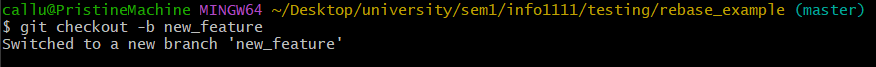
\includegraphics[width=1.1\textwidth]{rebasenewbranch}
\begin{itemize}
\item Adding multiple commits to the new branch
\end{itemize}
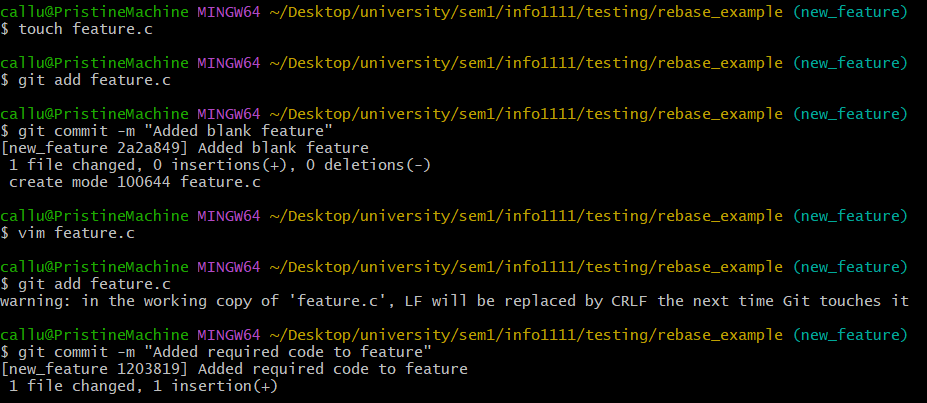
\includegraphics[width=1.1\textwidth]{rebasecommits}
\begin{itemize}
\item The new branch logs vs the master logs 
\end{itemize}

- New branch log

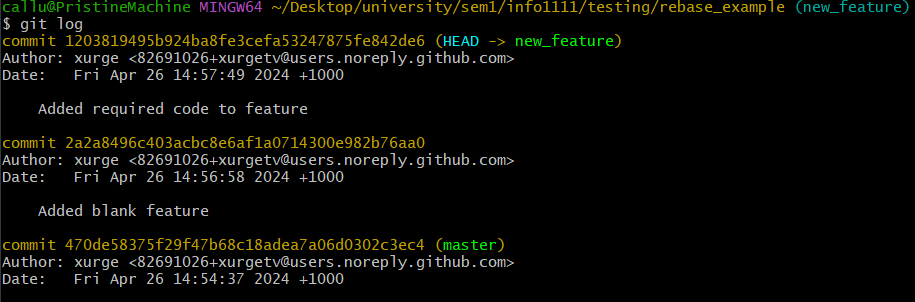
\includegraphics[width=1.1\textwidth]{rebasenewlogs}

- Master log

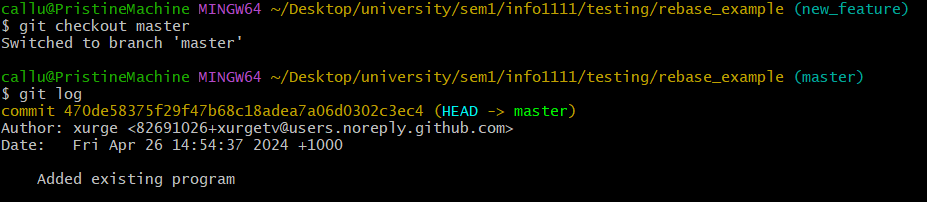
\includegraphics[width=1.1\textwidth]{rebasenewlogsmaster}
\begin{itemize}
\item Within the master, rebasing the new branch and seeing the now updated logs with commits from new branch
\end{itemize}
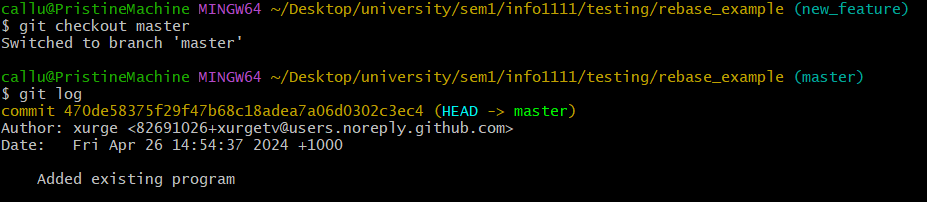
\includegraphics[width=1.1\textwidth]{rebaserebaselogcheck}
 
\vspace{\baselineskip}
 \textbf{Ignoring Files:}

A .gitignore file allows for a more efficient use of the git add command, allowing it to ignore specific files or file patterns that appear in the .gitignore file.  This  is useful for keeping the remote repository clean of temporary files, and reducing the risk of uploading sensitive data. 

Below is an example: 


\begin{itemize}
\item View of starting files in repository 
\end{itemize}
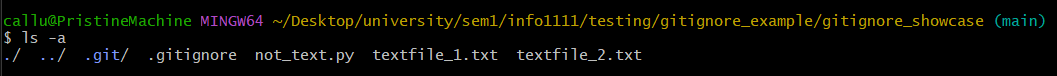
\includegraphics[width=1.1\textwidth]{gitignorestartingfiles}
\begin{itemize}
\item Using git status to see all unstaged files that have been created or changed 
\end{itemize}
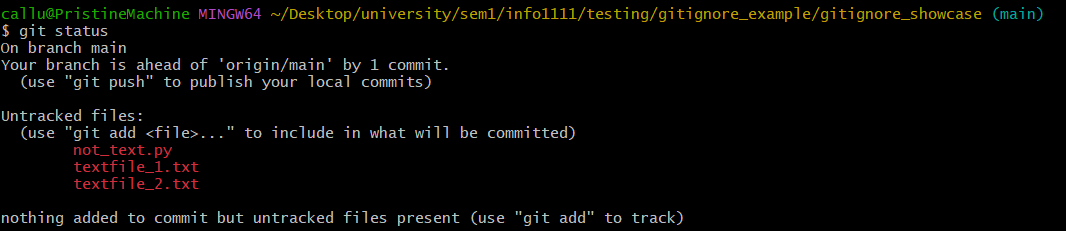
\includegraphics[width=1.1\textwidth]{gitignoreinitialstatus}
\begin{itemize}
\item Adding a pattern into the .gitignore file that ignores all files with txt extension  
\end{itemize}
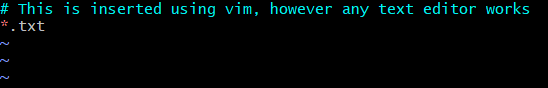
\includegraphics[width=1.1\textwidth]{gitignorevim}
\begin{itemize}
\item Git adding and committing the .gitignore file 
\end{itemize}
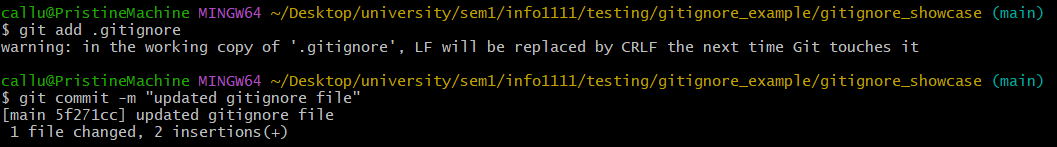
\includegraphics[width=1.1\textwidth]{gitignorecommit}
\begin{itemize}
\item Checking the status of the repository again shows all txt files are no longer included in tracking for next commit check 
\end{itemize}
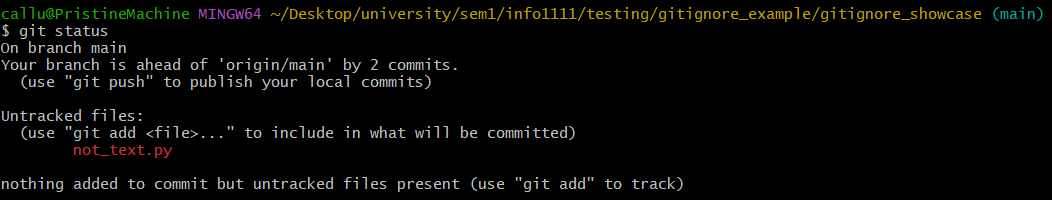
\includegraphics[width=1.1\textwidth]{gitignorefinalstatus}
\begin{itemize}
\item Now using commands that normally add and commit all changed or created files 
\end{itemize}
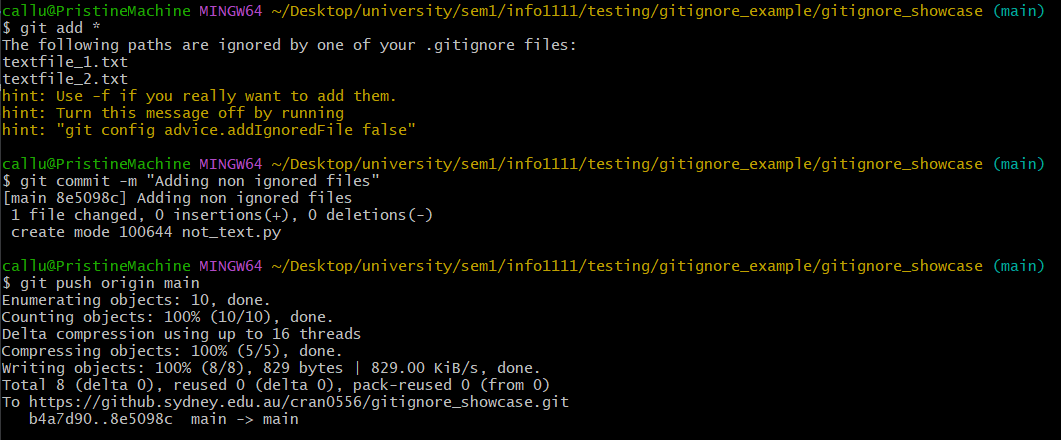
\includegraphics[width=1.1\textwidth]{gitignoreaddall}
\begin{itemize}
\item Can see the remote repository did not receive ignore files in commit 
\end{itemize}
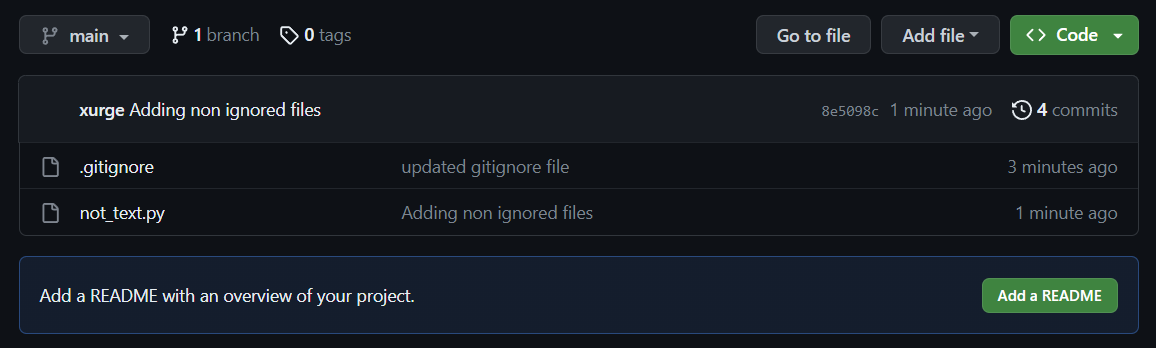
\includegraphics[width=1.1\textwidth]{gitignorerepo}

\vspace{\baselineskip}
 \textbf{\large{LaTeX Skill: Cross-referencing and Custom Commands}}

\vspace{\baselineskip}
 \textbf{Cross-referencing:}

Cross-referencing allows for text to be linked to section, figures, equations, etc., each with their own numbers and bracket formatting, allowing for a clear indication of what information is being referred to in text. This is done through the \verb|\label{type:name}| and \verb|\ref{type:name}| commands, ensuring that the name in both is the same. It is important that the type exists in the correct environment or on the line of code that is is refering to. This pattern can be seen in action in the following:

- I use the fig: type here \ref{fig:figureexample} along with an environment to apply appropriate labling and brackets and numbering. 

\begin{figure}[htbp]
    \centering
    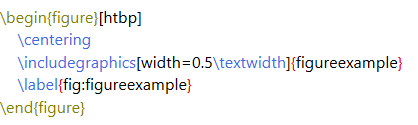
\includegraphics[width=0.5\textwidth]{figureexample}
    \label{fig:figureexample}
\end{figure}

- Now here is a cross-reference to a figure again, but we will refer to it as a table (sourced from \cite{labletypes}). The table displays all the different types of lables \ref{table:tableexample} Notice that it also has the lable 2.1. This indicates that the referenced material is in section 2.1 of the latex document.
 
\begin{table}[htbp]
    \centering
    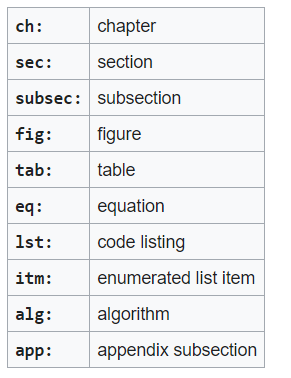
\includegraphics[width=0.5\textwidth]{tableexample}
    \label{table:tableexample}
\end{table}

\vspace{\baselineskip}
 \textbf{Custom Commands:}

\newcommand{\bigred}[1]{
	\textcolor{red}{\large #1}
}

The benefits of using \verb|\newcommand|, is that it allows for the defining of otherwise tedious, or space consuming commands to be used under a new name, such as a command that makes text large and red. This can be done \bigred{like so}. Here is what's happening:

- The command

 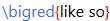
\includegraphics[width=0.23\textwidth]{mycommand}

\vspace{\baselineskip}
- The code

 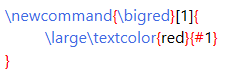
\includegraphics[width=0.4\textwidth]{commandcode}

\vspace{\baselineskip}
Breaking done what is happening here: \\
\noindent This is done by first giving the new command a name in curly brackets following the  \verb|\newcommand\{name here\}|. From here another set of curly brackets holds the commands that you want to perform. If you require input into your command, place square brackets between the sets of curly brackets like this:

\verb|\newcommand{name}[number of inputs]{command description}|, 

which then holds the number of inputs you require. To then refer to these inputs, you must use the order they appear in after a hastag, following this exampple. See how there are two inputs, one in the first curly brackets, and one in the next. The first text provided in refered to in the first line of new command descriptor and makes the text blue, referring with \#1. Whereas the second input is referred to with \#2, and is used in the second line to make the text red. 


% ========================================================

\subsection{Tools and Skills for \majB: \studB}

\textbf{\large{Part A: Exploration of Tech Tools}}

\textbf{\large{Tool Identification}}

In the field of data science, I have chosen R and SQL, two highly practical tools that are widely used by data scientists. These tools are essential due to their powerful functionalities in data analysis, management, and statistical computation, making them indispensable in the industry.

\vspace{\baselineskip}

\textbf{\large{Tool 1 Questions - R}}

\textbf{Question 1: What is the main function of R in the field of data science, in 250 words or less?}

R is a programming language and software environment specifically designed for statistical computing and graphics. Its primary function in data science is to provide a comprehensive suite of tools that facilitate data manipulation, statistical analysis, and visualization.

R offers a vast array of statistical tests and models, enabling data scientists to perform complex analyses, from basic descriptive statistics to advanced inferential techniques. The language's built-in functions and extensive package ecosystem support a wide range of statistical methodologies, making it an ideal tool for researchers and analysts.

R's powerful data visualization capabilities, particularly through the ggplot2 package, allow for the creation of high-quality, customizable plots that help in exploring and presenting data insights. Additionally, R provides robust data manipulation tools, such as the dplyr and tidyr packages, which streamline the process of cleaning and transforming data for analysis.

These features make R a versatile tool that supports the entire data analysis workflow, from data preparation and exploration to modeling and reporting, ensuring that data scientists can efficiently derive meaningful insights from their data.

\vspace{\baselineskip}

\textbf{Question 2: How is R used in the data science industry, in 250 words or less?}

R is extensively used in the data science industry for a variety of applications across different sectors.

In academia and research, R is a preferred tool for conducting statistical analyses and hypothesis testing, thanks to its comprehensive statistical functions and reproducibility. Researchers utilize R to develop new statistical methods and to publish detailed analytical results.

In the pharmaceutical industry, R is critical for analyzing clinical trial data, aiding in drug development and ensuring regulatory compliance. Bioinformatics professionals use R for analyzing genomic data, performing sequence analysis, and developing predictive models for biological phenomena.

The finance sector also heavily relies on R for risk modeling, portfolio optimization, and quantitative analysis, where accurate statistical analysis is crucial. Businesses leverage R to build predictive models that forecast sales, customer behavior, and market trends, facilitating data-driven decision-making.

R's ability to handle complex statistical tasks and its extensive library of packages tailored for various analytical needs make it a vital tool in the data science industry, enabling professionals to tackle diverse data challenges effectively.

\vspace{\baselineskip}

\textbf{Question 3: Does R have any weaknesses or limitations, in 250 words or less?}

Yes, R has several weaknesses and limitations.

One major limitation is its memory management. R often requires loading entire datasets into memory, which can be problematic when dealing with very large datasets. This limitation can lead to performance issues, as processing large datasets may require substantial RAM, which might not be available on standard personal computers. Consequently, R's performance can degrade significantly with increasing data size, leading to slower computations and potential crashes.

Another limitation of R is its steep learning curve, especially for users who are not familiar with programming or statistical analysis. The extensive range of functions and packages can be overwhelming for beginners, making it challenging to navigate and utilize R effectively without substantial time and effort invested in learning.

Additionally, while R excels in statistical analysis and visualization, it may not be as efficient for general-purpose programming tasks or large-scale data processing compared to other languages like Python. These weaknesses highlight the need for careful consideration when choosing R for specific data science tasks, ensuring that its strengths align with the project requirements and available resources.

\vspace{\baselineskip}

\textbf{\large{Tool 2 Questions - SQL}}

\textbf{Question 1: What is the main function of SQL in the field of data science, in 250 words or less?}

SQL, which stands for Structured Query Language, is a specialized programming language designed for managing and manipulating relational databases. Its primary function in data science is to facilitate the efficient querying, updating, and management of structured data stored in relational databases.

SQL allows data scientists to perform complex queries to filter, sort, and aggregate data, enabling them to extract valuable insights from large datasets. The language's straightforward syntax makes it easy to write and understand queries, which helps in retrieving specific data needed for analysis.

SQL supports various operations such as data insertion, updating, and deletion, ensuring data integrity and consistency through the use of constraints and transactions. Additionally, SQL's aggregate functions, such as SUM, AVG, COUNT, MAX, and MIN, allow for effective statistical analysis directly within the database, making it a powerful tool for generating reports and summarizing data.

Overall, SQL's robust capabilities in managing and querying structured data make it an essential tool for data scientists who need to work with large and complex datasets stored in relational databases.

\vspace{\baselineskip}

\textbf{Question 2: How is SQL used in the data science industry, in 250 words or less?}

SQL is widely used in the data science industry for managing and analyzing structured data across various sectors.

In the finance industry, SQL is essential for handling large volumes of transactional data, customer records, and financial information. Financial analysts use SQL to query databases for real-time insights, generate financial reports, and perform risk analysis.

In the retail sector, SQL helps manage inventory, track sales, and analyze customer data, providing valuable insights for optimizing stock levels and personalizing marketing strategies. SQL is also crucial in healthcare, where it is used to manage patient records, clinical data, and research information, enabling healthcare professionals to conduct data-driven research and improve patient care.

In technology companies, SQL is used for managing big data generated by applications, websites, and IoT devices. Data engineers and analysts use SQL to process and analyze this data, integrating it with other data processing tools to create comprehensive data workflows.

SQL's ability to handle structured data efficiently and its compatibility with various database systems make it a versatile and indispensable tool in the data science industry, facilitating data management, analysis, and reporting across different domains.

\vspace{\baselineskip}

\textbf{Question 3: Does SQL have any weaknesses or limitations, in 250 words or less?}

Yes, SQL has several weaknesses and limitations.

One of the main limitations of SQL is its limited expressive power when dealing with complex unstructured data. SQL is designed primarily for structured data and excels in managing and querying relational databases, but it struggles with unstructured data such as text, images, and videos. Handling such data often requires additional tools or languages, such as NoSQL databases, which are better suited for managing unstructured data.

Another limitation is performance overhead. While SQL queries are efficient for structured data, complex queries on large datasets can lead to performance bottlenecks, requiring optimization of database structures, indexing, and query tuning. Ensuring compatibility between different versions of SQL and database systems can also pose challenges, particularly in large-scale deployments with diverse environments.

Additionally, SQL’s reliance on a predefined schema can be restrictive in scenarios where data models need to evolve quickly. Schema changes can be cumbersome and may require significant modifications to existing queries and applications.

Despite these limitations, SQL remains a powerful tool for managing and querying structured data, but its effectiveness can be enhanced when used in conjunction with other technologies that address its weaknesses.

\subsubsection{Part B: Analysis}

\textbf{\large{Tool 1 Response Evaluation - R}}

\textbf{Functionality of R:} \\
\noindent I agree with this answer. It rightly highlights the main functions of R in data science, including statistical analysis, data manipulation, and visualization. The mention of specific packages such as ggplot2 for visualization and dplyr and tidyr for data manipulation emphasizes R's strengths in handling diverse data science tasks. This answer effectively summarizes R's comprehensive capabilities and clearly illustrates why R is the tool of choice in data science.

\textbf{Usage of R in the Data Science Industry:} \\
\noindent I agree with this answer. It accurately describes how R is used in different industries, demonstrating its versatility. Also, R is a popular choice among data scientists and is used by many organizations, including Fortune 500 companies, government agencies, and top research institutions.\cite{Linkedin} The examples provided—academia, pharmaceutical industry, bioinformatics, finance, and business—are relevant and highlight the wide range of applications for R. The answer is very well written and organized. Emphasis on R's ecosystem of packages further demonstrates its adaptability and effectiveness in handling specific analytical needs. This answer is comprehensive and in line with practical applications of R in the data science industry.

\textbf{Weaknesses or Limitations of R:} \\
\noindent I agree with this answer. It rightly points out the significant limitations of R, including memory management issues and a steep learning curve. For example, a large and varied set of built-in functions is not enough to do all the cool things you can do with R, from plotting compelling data visualizations to training powerful machine learning models.\cite{DataCamp} The difference between R's strengths in statistical tasks and its inefficiencies in general-purpose programming or large-scale data processing has been well pointed out. These limitations are critical considerations for anyone choosing to use R for a data science project, ensuring that users understand the challenges they may face.

\vspace{\baselineskip}\\
\noindent \textbf{\large{Tool 2 Response Evaluation - SQL}}

\textbf{Functionality of SQL:} \\
\noindent I agree with this answer. It succinctly explains the main functions of SQL in data science, focusing on its ability to manage and query structured data in relational databases. SQL server functions are pre-built actions that perform calculations, manipulate data, and return results. At the most fundamental level, these functions simplify complex queries and automate repetitive tasks.\cite{blogs} References to SQL's simple syntax and ability to perform statistical analyses directly in a database emphasized its usefulness and efficiency. The answer effectively communicates the primary role of SQL and its importance in working with structured data.

\textbf{Usage of SQL in the Data Science Industry:} \\
\noindent I agree with this answer. It provides a clear and comprehensive overview of the use of SQL in different industries, emphasizing its versatility and efficiency in managing structured data. SQL is extremely important for data science. It allows you to work with structured data stored in databases. As a data scientist, you need SQL to extract, manipulate, and analyze data from these databases. Big data tools like Hadoop and Spark also use SQL for processing structured data. Learning SQL skills like querying, joining tables, filtering, and aggregating data is crucial. Combining SQL with Python makes data management and analysis convenient without switching between languages. Whether dealing with relational databases or working with big data, mastering SQL is essential for any aspiring data scientist. It empowers you to wrangle, prepare, and gain insights from data effectively.\cite{Analytics}

\textbf{Weaknesses or Limitations of SQL:} \\
\noindent I agree with this answer. There are several weaknesses, including poor interface, cost inefficiency, partial control, and security concerns. 
Poor Interface: SQL has a poor interface, which makes things look very complex, even if they are not. Users find it difficult to deal with databases due to the difficulty of using the SQL interface.
Cost Inefficiency: SQL Server Standard costs around \verb|$|1,418/year. The high cost makes it difficult for some programmers to use it.
Partial Control: SQL doesn't grant its users complete control over databases due to some hidden business rules. This can be a huge drawback for many.
Security: Regardless of the SQL version, databases in SQL are constantly under threat as they hold huge amounts of sensitive data.\cite{Unstop}

\subsubsection{Technical Skills (LaTeX and Git)}
\textbf{\large{Git Skills: Forking and Special Files}}\\
\textbf{Forking:}
\noindent Forking is a common form of collaborative development that allows developers to develop independently without affecting the original project. Forking gives you the freedom to experiment and improve your project, and when you're done, you can submit your changes to the original project via pull request for code merging.

\noindent There are two ways to create a fork. The one way is clicking the ‘fork’ button in Github and creating it.
\begin{center}
	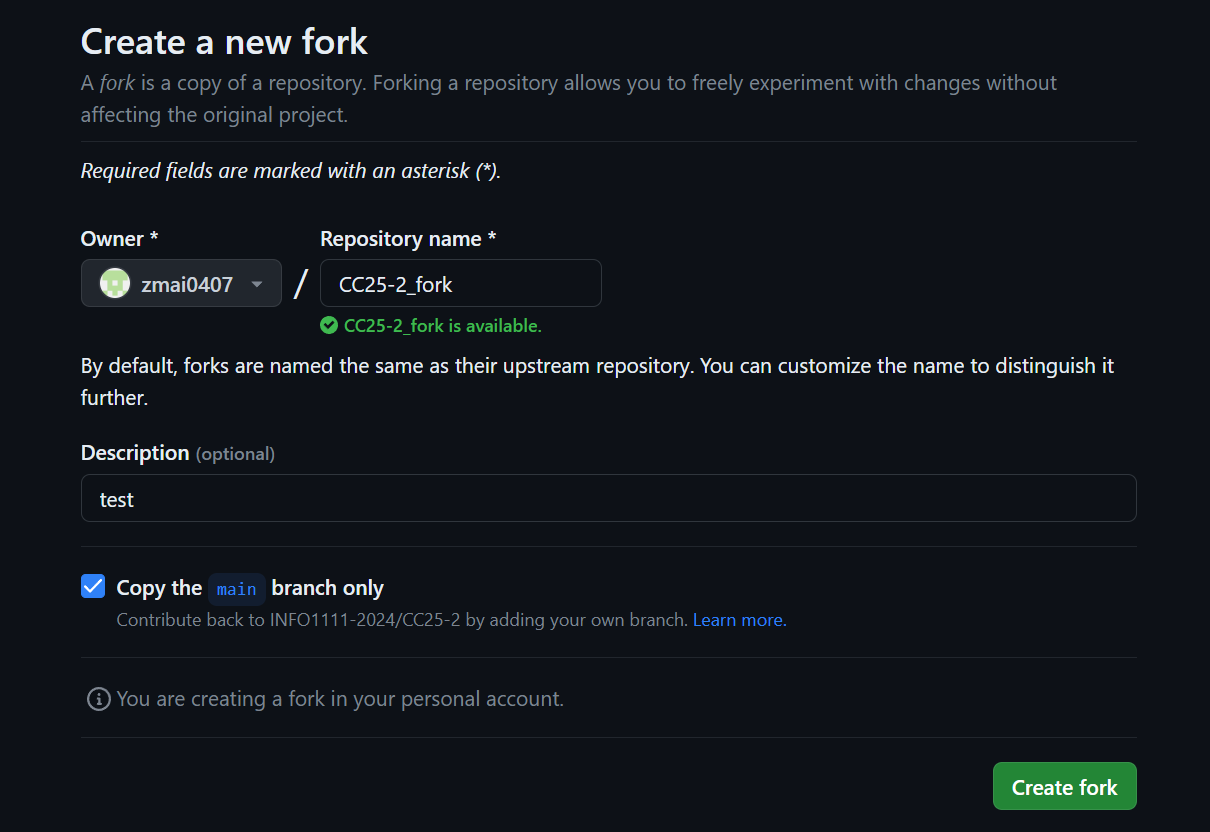
\includegraphics[width=0.8\textwidth, keepaspectratio]{createanewfork_ingithub}
\end{center}


\begin{center}
	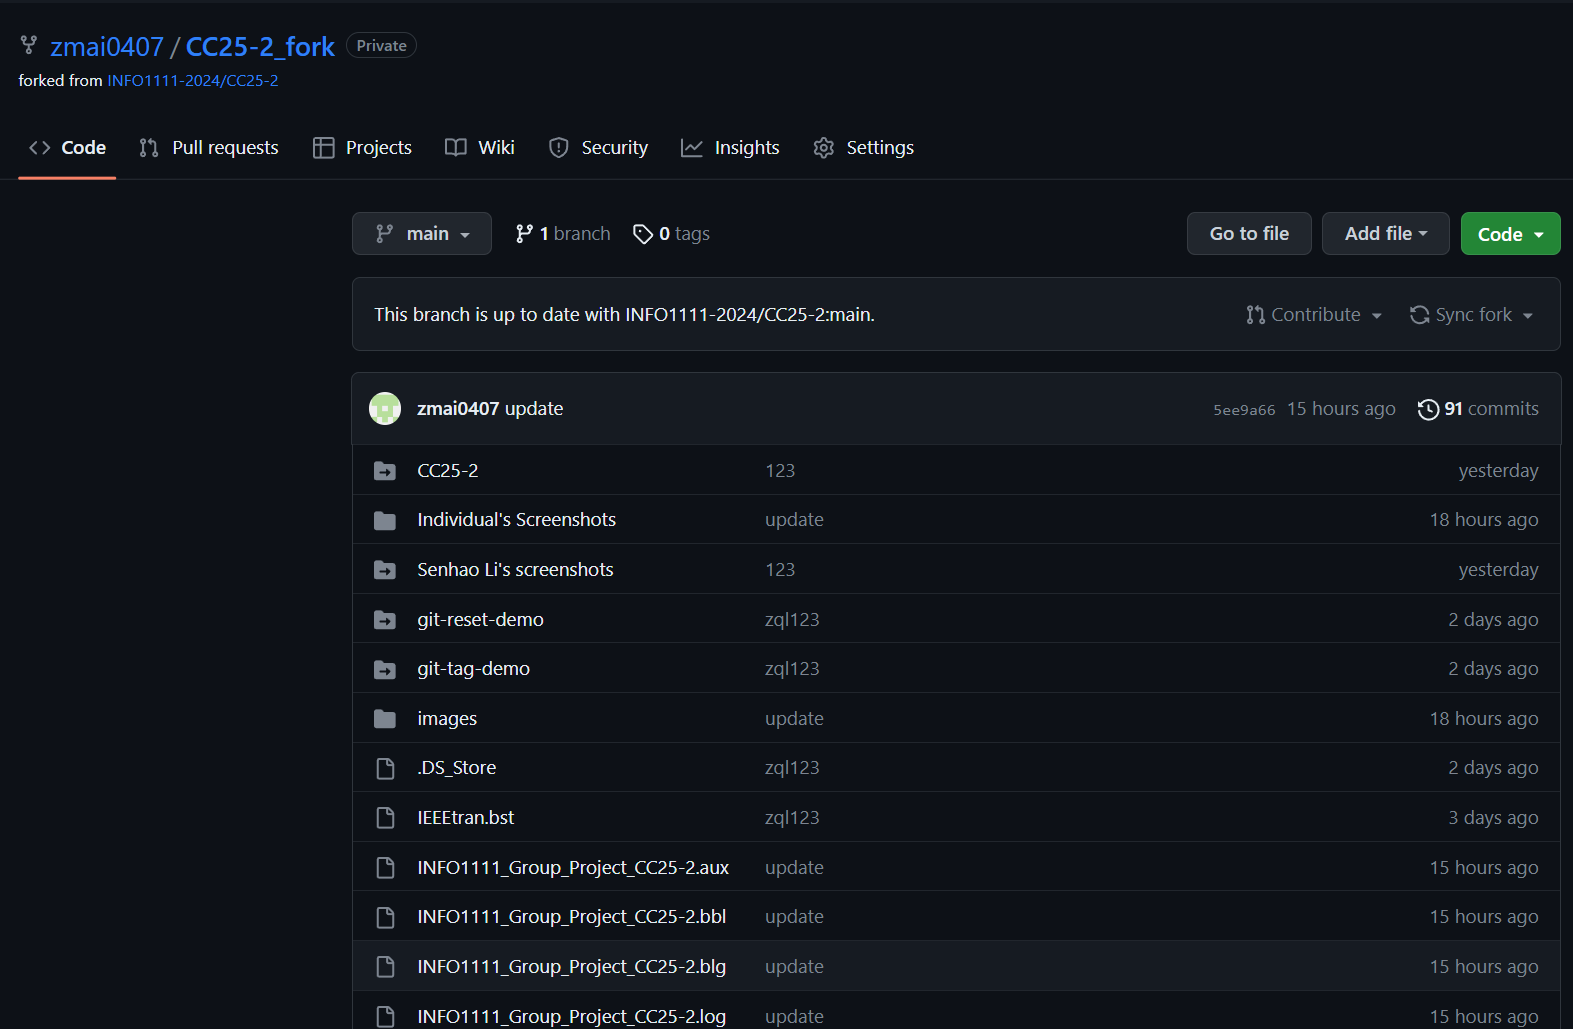
\includegraphics[width=0.8\textwidth, keepaspectratio]{anewfork_ingithub}
\end{center}


\noindent And another way is creating a fork in git.\\
Firstly, I create a new repository in github.
\begin{center}
	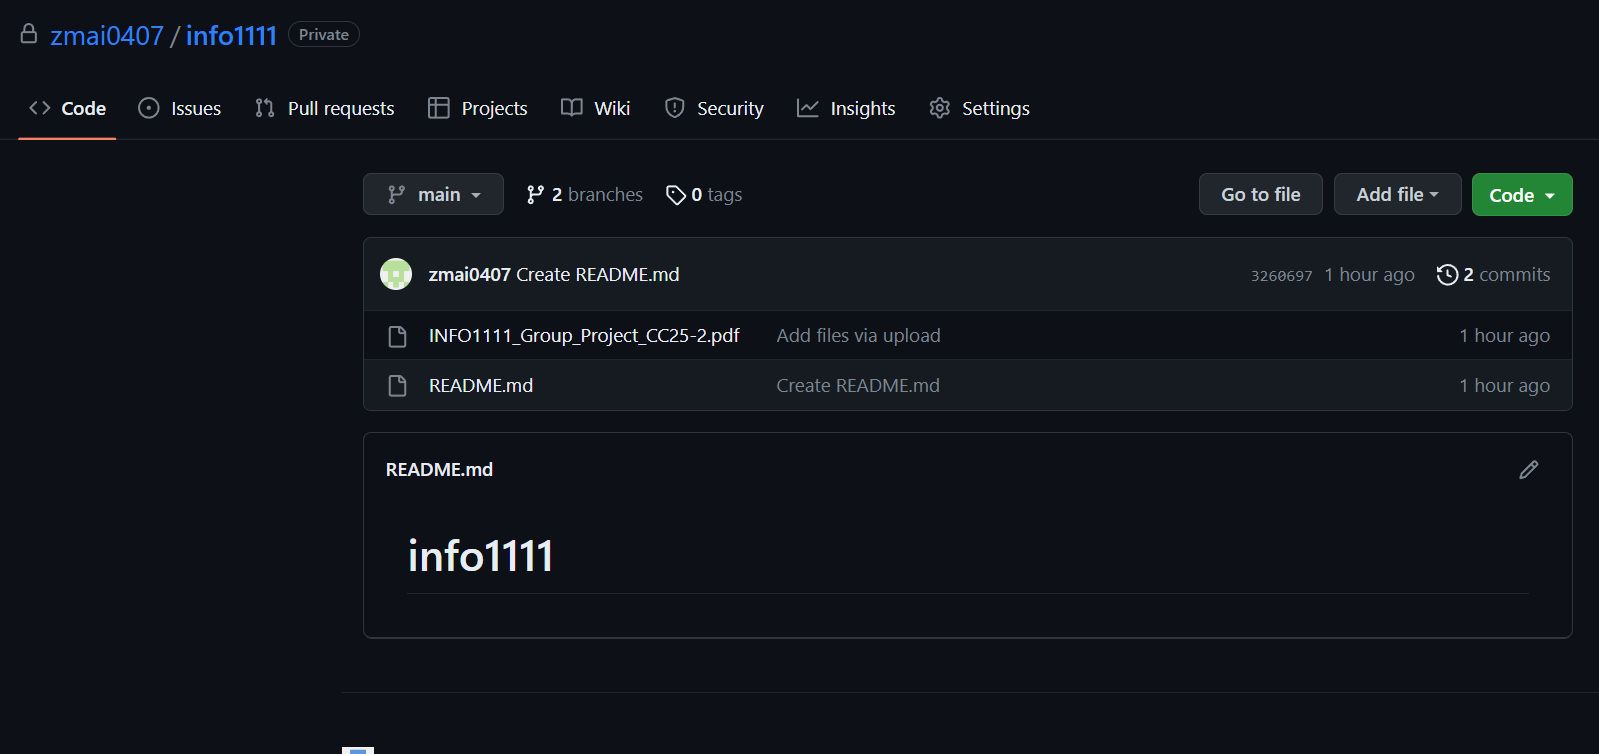
\includegraphics[width=0.8\textwidth, keepaspectratio]{newrepository}
\end{center}


\noindent Secondly, I cloned the original repository locally and added a new remote repository.
\begin{center}
	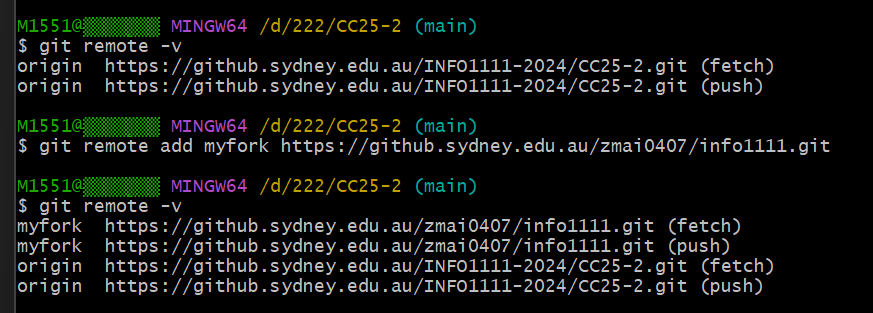
\includegraphics[width=0.8\textwidth, keepaspectratio]{repository_ingit}
\end{center}


\noindent Then I created a new branch for independent development. 
\begin{center}
	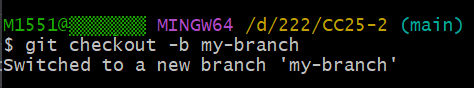
\includegraphics[width=0.8\textwidth, keepaspectratio]{addnewbramch}
\end{center}


\noindent After making changes and commits on the new branch,I pushed the new branch to the remote repository and committed the changes to the original project via Pull Request for code review and merge.
\begin{center}
	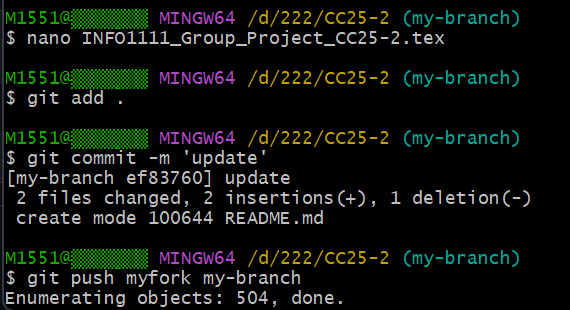
\includegraphics[width=0.8\textwidth, keepaspectratio]{pushnewchange}
\end{center}


\noindent Finally, I can find the compare \verb|&| pull request in Github.
\begin{center}
	\includegraphics[width=0.8\textwidth, keepaspectratio]{Compareandpullrequest}
\end{center}

\begin{center}
	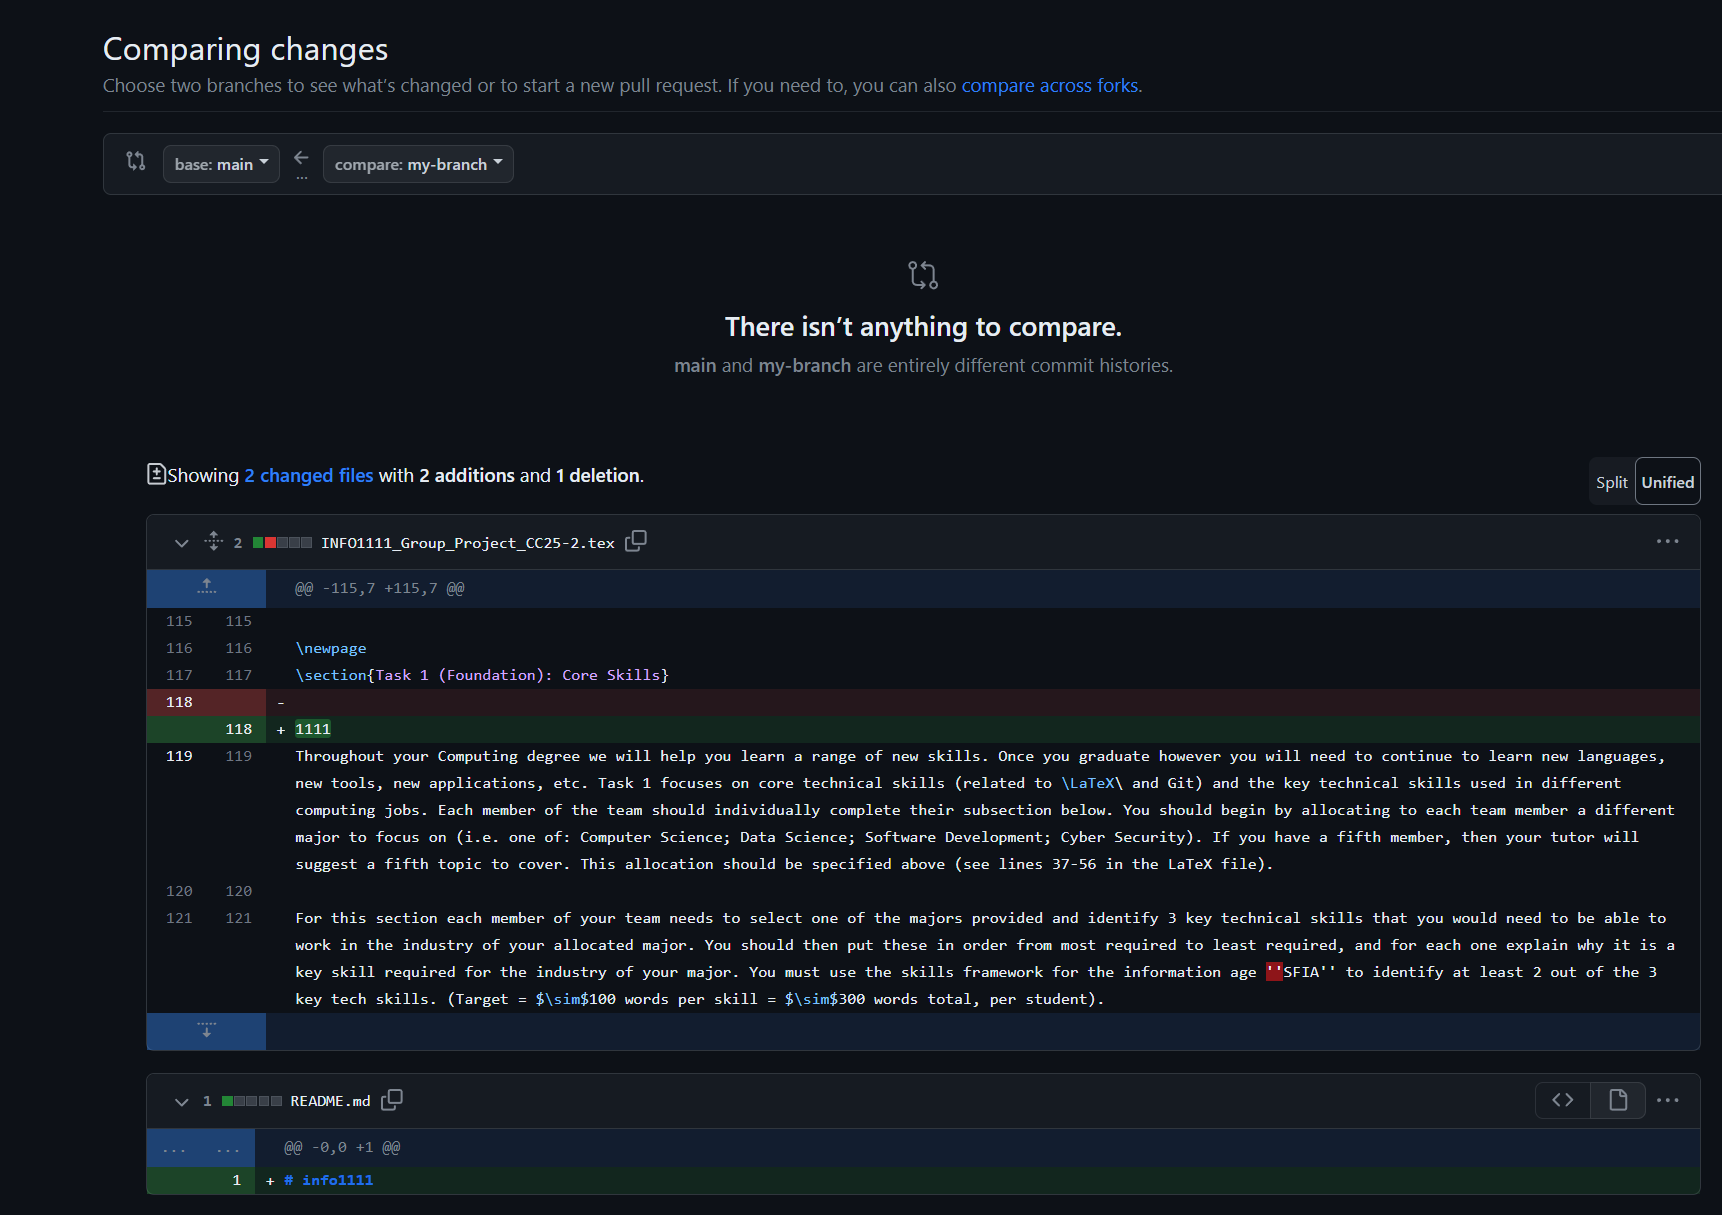
\includegraphics[width=0.8\textwidth, keepaspectratio]{compare}
\end{center}

\textbf{Special Files:}
\noindent In Git, Special Files refer to configuration files with specific purposes that help you manage and control the behavior of your Git repository. Common special files include .gitignore and .gitattributes, but there are other special files: 
\begin{center}
	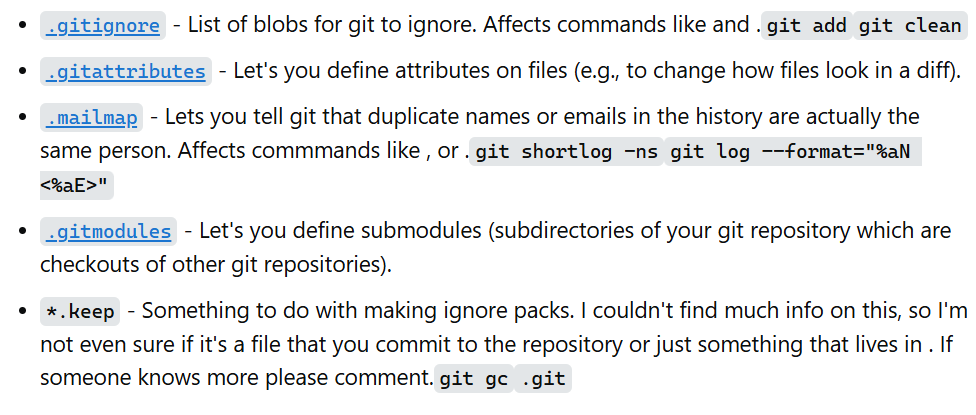
\includegraphics[width=0.8\textwidth, keepaspectratio]{specialfile.png}
\end{center}

\noindent .gitignore: Specifies which files or directories Git should ignore and not include in version control. This is useful for excluding temporary files, compilation output, and sensitive information.
-Ignore all .log, .class and .lock files
\begin{center}
	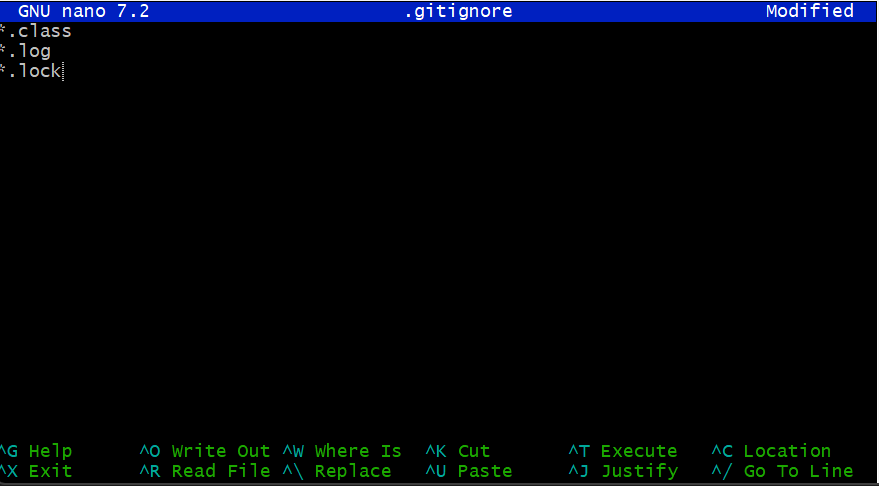
\includegraphics[width=0.8\textwidth, keepaspectratio]{nanoignore.png}
\end{center}
-add .gitignore to the staging area
\begin{center}
	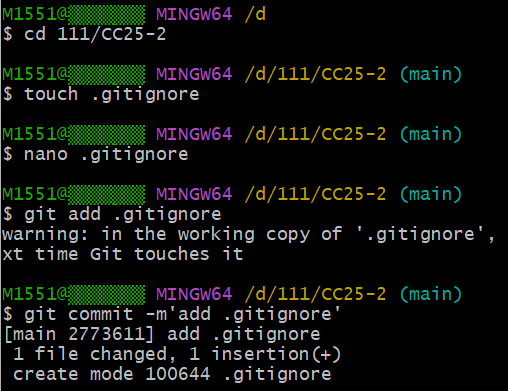
\includegraphics[width=0.8\textwidth, keepaspectratio]{ignore.png}
\end{center} 
\noindent .gitattributes: Defines file attributes that control how Git handles these files. This can be used to specify line terminators for text files, merge policies, etc. 
-Set all text files to use LF line endings and Mark .jpg files as binary
\begin{center}
	\includegraphics[width=0.8\textwidth, keepaspectratio]{nanoattributes.png}
\end{center}
-add .gitattributes to the staging area
\begin{center}
	\includegraphics[width=0.8\textwidth, keepaspectratio]{attributes.png}
\end{center}
-the result of uploading with lots files
\begin{center}
	\includegraphics[width=0.8\textwidth, keepaspectratio]{complete2.png}
\end{center}
-the .log file is not uploaded(be ignored).
\begin{center}
	\includegraphics[width=0.8\textwidth, keepaspectratio]{complete1.png}
\end{center}

\textbf{\large{LaTeX Skill: Footnotes/margin notes and creating new environments}}
\textbf{Footnotes:}
Footnotes allow for the addition of supplementary information or references at the bottom of the page, providing readers with additional context without interrupting the main text flow. This is accomplished using the \verb|\footnote{}| command, where the text inside the braces appears as a numbered footnote at the bottom of the page. Just like that:

\begin{center}
\includegraphics[width=1.0\textwidth, keepaspectratio]{ZIXI_MAI_footnote.png}
\end{center}

\textbf{Margin notes:}
Margin notes, on the other hand, offer a way to add brief comments or explanations in the page margins, making them visible alongside the main text. This can be achieved with the \verb|\marginnote{}| command, positioning the note in the right margin by default.

\begin{center}
\includegraphics[width=1.0\textwidth, keepaspectratio]{ZIXI_MAI_marginnote.png}
\end{center}

\textbf{Creating a new environment:}
Additionally, creating new environments in LaTeX allows for the definition of custom formatting for specific sections of text. This is done using the \verb|\newenvironment{name}{begin-code}{end-code}| command, where \verb|name| is the name of the new environment, and \verb|begin-code| and \verb|end-code| specify the formatting to apply at the start and end of the environment, respectively. These tools enhance document readability and organization, as illustrated below:

\begin{center}
\includegraphics[width=1.0\textwidth, keepaspectratio]{ZIXI_MAI_newenvironment.png}
\end{center}

And I put all the commands together (here is the example of bfseries):

\begin{center}
\includegraphics[width=0.8\textwidth, keepaspectratio]{ZIXI_MAI_example.png}
\end{center}

\begin{center}
\includegraphics[width=1.0\textwidth, keepaspectratio]{ZIXI_MAI_examplepdf.png}
\end{center}

% ========================================================

\subsection{Tools and Skills for \majC: \studC}

\subsubsection{Part A: Exploration of tech tools}

\textbf{\large{Tool Identification}}

In the field of software development, I have chosen Xcode and pycharm, two very practical tools that are widely used by software developers. I am certain that this is a software that software development professionals often need, and due to its convenience and powerful functionality, it has been widely used in practice.

\vspace{\baselineskip}
\textbf{\large{Tool 1 Questions - Xcode}}

\textbf{Question 1: What is the main function of Xcode in the field of software development, using 250 words or less?}

Xcode is an Integrated Development Environment (IDE) developed by Apple Inc. specifically for creating applications for Apple's platforms, including macOS, iOS, watchOS, and tvOS. Its primary function in software development is to provide a comprehensive suite of tools that facilitate the entire development process from coding to deployment.

Xcode's sophisticated code editor supports languages such as Swift and Objective-C, offering features like syntax highlighting, code completion, and real-time error checking, which significantly enhance coding efficiency and accuracy. The built-in debugger allows developers to inspect code execution in real-time, set breakpoints, and monitor variable states, enabling effective troubleshooting and optimization.

A standout feature of Xcode is its Interface Builder, a visual design tool that allows developers to create and test user interfaces using a drag-and-drop interface. This tool streamlines the design process and ensures a cohesive user experience across different devices.

Additionally, Xcode includes performance analysis tools like Instruments, which help developers profile and optimize their applications, ensuring they run smoothly and efficiently. The IDE also integrates extensive documentation and resources, providing developers with the necessary information and support throughout the development lifecycle.

Overall, Xcode's main function is to offer an all-encompassing environment that supports the development, debugging, and deployment of applications within the Apple ecosystem, making it an indispensable tool for developers targeting Apple platforms.
\vspace{\baselineskip}

\textbf{Question 2: How is Xcode used in the software development industry, in 250 words or less?}

Xcode is extensively used in the software development industry for creating applications across Apple’s ecosystem, including macOS, iOS, watchOS, and tvOS. It serves as the primary development environment for developers targeting these platforms due to its comprehensive toolset and seamless integration with Apple’s software and hardware.

Developers use Xcode to write code in Swift and Objective-C, leveraging its advanced code editor for efficient and error-free programming. The IDE’s real-time error detection and code completion features significantly speed up the coding process, allowing developers to quickly identify and fix issues.

Xcode’s Interface Builder is a key tool for designing user interfaces. It enables developers to create visually appealing and functional UIs through a drag-and-drop interface, ensuring a consistent user experience across different Apple devices. This visual approach to UI design helps streamline the development process and reduces the time required to create intuitive interfaces.

The built-in debugger in Xcode is crucial for testing and troubleshooting applications. Developers can set breakpoints, monitor variable states, and step through code to identify and resolve bugs effectively. Additionally, Xcode’s Instruments tool provides performance analysis, helping developers optimize their applications for better performance and resource management.

In the industry, Xcode is essential for deploying applications to the Apple App Store. It provides all the necessary tools for compiling, testing, and submitting apps, ensuring they meet Apple’s stringent quality standards.

Overall, Xcode’s integration of coding, debugging, UI design, and performance optimization tools makes it an indispensable environment for professional developers focused on Apple platforms.

\vspace{\baselineskip}
\textbf{Question 3: Does Xcode have any weaknesses or limitations, in 250 words or less?}

Yes, Xcode has several weaknesses and limitations. Xcode is exclusive to macOS, meaning it can only be used on Apple computers. This limits accessibility for developers using other operating systems, such as Windows or Linux, requiring them to invest in Apple hardware if they want to develop applications for Apple's platforms.

Xcode is resource-intensive, demanding significant memory and processing power to run smoothly. On older or less powerful machines, Xcode can be slow and unresponsive, hindering the development process and reducing productivity.

For beginners, Xcode has a steep learning curve. Its extensive range of features and tools can be overwhelming, making it difficult for new developers to navigate and utilize effectively. While comprehensive documentation is available, the complexity of the IDE remains a challenge for those unfamiliar with Apple's development environment.

Performance and stability issues are common complaints. The IDE can sometimes crash or exhibit bugs, especially with new releases or updates. These issues disrupt the development workflow and require time to troubleshoot and resolve.

Xcode's integration with non-Apple technologies and platforms is limited. This can be a disadvantage for developers working with cross-platform tools or frameworks, as they may encounter compatibility issues or lack of support within the Xcode environment.

Overall, while Xcode is a powerful and essential tool for developing applications within the Apple ecosystem, its platform exclusivity, resource demands, steep learning curve, and occasional stability issues are notable limitations.

\vspace{\baselineskip}
\textbf{\large{Tool 2 Questions - Pycharm}}

\textbf{Question 1: What is the main function of Pycharm in the field of software development, using 250 words or less?}

PyCharm is an Integrated Development Environment (IDE) specifically designed for Python programming, developed by JetBrains. Its primary function in software development is to provide a comprehensive suite of tools that facilitate efficient coding, debugging, and project management for Python developers.

PyCharm offers an intelligent code editor that supports advanced features such as syntax highlighting, code completion, and real-time error detection, which significantly enhance coding accuracy and efficiency. The IDE also includes a powerful debugger that allows developers to inspect and control code execution, set breakpoints, and evaluate expressions, enabling effective troubleshooting and optimization.

One of PyCharm's key functionalities is its integration with popular web frameworks such as Django and Flask. This integration simplifies web development by providing dedicated tools, templates, and support for these frameworks, making it easier to develop, test, and deploy web applications.

PyCharm also includes built-in tools for database management and querying, which streamline interactions with databases directly from the IDE. This feature is particularly useful for data-intensive applications and projects that require seamless database integration.

Additionally, PyCharm supports version control systems like Git, allowing developers to manage their code repositories, track changes, and collaborate with team members efficiently. The IDE’s comprehensive support for testing frameworks helps ensure code quality by facilitating the writing, running, and debugging of unit tests.

Overall, PyCharm’s main function is to provide a robust, all-encompassing development environment that enhances productivity, code quality, and project management for Python developers.

\vspace{\baselineskip}
\textbf{Question 2: How is Pycharm used in the software development industry, in 250 words or less?}

PyCharm is widely used in the software development industry for various types of Python projects, including web development, data science, machine learning, automation, and scripting. Its robust set of features and tools makes it a popular choice among developers and organizations aiming to improve coding efficiency, maintain high code quality, and streamline project workflows.

In web development, PyCharm's integration with popular frameworks such as Django, Flask, and Pyramid simplifies the development process. It provides built-in templates, project scaffolding, and debugging tools that help developers quickly build, test, and deploy web applications. PyCharm's support for front-end technologies like HTML, CSS, and JavaScript further enhances its utility for full-stack development.

For data science and machine learning, PyCharm offers excellent support for libraries such as NumPy, pandas, Matplotlib, and TensorFlow. Its scientific mode provides an interactive environment similar to Jupyter Notebooks, allowing data scientists to analyze data, visualize results, and experiment with machine learning models efficiently.

PyCharm is also valuable for automation and scripting tasks. Its intelligent code editor, combined with powerful debugging and testing tools, enables developers to write and maintain scripts that automate repetitive tasks, improving productivity and reducing errors.

Additionally, PyCharm's built-in version control system (VCS) integration, particularly with Git, facilitates efficient collaboration among development teams. It allows developers to manage code repositories, track changes, and resolve conflicts seamlessly within the IDE.

Overall, PyCharm is a versatile tool that supports a wide range of Python development activities, making it indispensable for developers and organizations seeking to optimize their software development processes.

\vspace{\baselineskip}
\textbf{Question 3: Does Pycharm have any weaknesses or limitations, in 250 words or less?}

Yes, PyCharm has several weaknesses and limitations. One of the primary issues is its resource intensity. PyCharm can be demanding on system resources, particularly when working with large projects or multiple plugins. This can lead to slower performance on less powerful machines, which may hinder productivity.

Another limitation is the cost associated with the professional edition. While PyCharm offers a free community edition, it lacks many advanced features available in the paid version. These features, such as full support for web development frameworks and advanced database tools, are crucial for many professional developers. The cost of the professional edition might be a barrier for individual developers or small teams with limited budgets.

For beginners, PyCharm's extensive feature set can be overwhelming. The IDE's complexity may pose a steep learning curve for new developers, making it challenging to navigate and utilize its full potential effectively. Despite comprehensive documentation and tutorials, the initial setup and configuration can be daunting.

Additionally, while PyCharm excels in Python development, it is less suitable for projects involving multiple languages or non-Python technologies. Developers working on polyglot projects might find PyCharm’s support for other languages limited compared to more general-purpose IDEs.

Lastly, occasional stability issues and bugs can disrupt the development workflow. Although JetBrains regularly updates PyCharm to address these issues, they can still affect user experience and productivity.

Overall, while PyCharm is a powerful and feature-rich IDE for Python development, its resource demands, cost, complexity for beginners, limited multi-language support, and occasional stability issues are notable limitations.

\subsubsection{Part B: Analysis}

\textbf{\large{Tool 1 Response Evaluation - Xcode}}

\textbf{Functionality of Xcode:} \\
\noindent I agree with ChatGPT's description of Xcode as an Integrated Development Environment (IDE) designed for Apple platforms like macOS, iOS, watchOS, and tvOS. The explanation of its primary function, including coding, debugging, and deployment, is thorough and highlights key features like the code editor, debugger, Interface Builder, and performance tools.\cite{wentk2014xcode}. However, it could mention the potential limitations for developers who are used to more flexible or less tightly integrated environments. While Xcode's all-encompassing nature is a strength, it might also mean less flexibility compared to modular development tools.

\textbf{Usage of Xcode in the Software Development:} \\
\noindent The provided answer effectively captures how Xcode is used across the Apple ecosystem, from coding in Swift and Objective-C to designing interfaces with Interface Builder and deploying apps to the App Store. This explanation aligns well with industry practices. However, it could have addressed how the close integration with Apple's hardware and software, while advantageous, can also lead to challenges when new updates introduce bugs or require significant changes.\cite{ohland2016xcode} Additionally, the response could have considered how Xcode's strong focus on Apple's ecosystem might limit its adoption in more diverse or cross-platform development teams.

\textbf{Weaknesses or limitations of Xcode:} \\
\noindent I agree with the detailed identification of Xcode's weaknesses, such as its macOS exclusivity, high resource demands, steep learning curve, and performance issues.\cite{lin2022xcode} These points are all valid and reflect common concerns among developers. However, the answer could have been more nuanced by discussing how Apple's continuous updates and improvements to Xcode address some of these issues over time. It might also have been beneficial to consider how these limitations impact different types of developers differently, with beginners potentially struggling more than experienced developers who can better navigate the complexities of the tool.

Overall, while the answers are comprehensive and accurate, incorporating a bit more critical analysis and considering different perspectives would make the assessment even more insightful.

\vspace{\baselineskip}\\
\noindent \textbf{\large{Tool 2 Response Evaluation - Pycharm}}

\textbf{Functionality of Pycharm:} \\
\noindent I agree with the answer provided by ChatGPT. It accurately describes PyCharm as an Integrated Development Environment (IDE) designed specifically for Python programming. The explanation highlights its comprehensive suite of tools for efficient coding, debugging, and project management, which are key aspects of any robust IDE.\cite{hu2018deepgraph} The mention of advanced features like syntax highlighting, code completion, real-time error detection, and powerful debugging tools is appropriate. Additionally, the integration with popular web frameworks and support for database management, version control systems, and testing frameworks underline PyCharm’s versatility and effectiveness in enhancing productivity and code quality. However, the answer could further emphasize how PyCharm's focus on Python can limit its use in multi-language projects, reflecting a potential trade-off between specialization and versatility.

\textbf{Usage of Pycharm in the Software Development:} \\
\noindent The answer provides a comprehensive overview of PyCharm’s use across various Python projects, including web development, data science, machine learning, automation, and scripting. It rightly points out PyCharm’s integration with web frameworks like Django and Flask, support for data science libraries, and utilities for automation tasks.\cite{van2023hands} The mention of built-in version control system (VCS) integration and its benefits for team collaboration is also accurate. However, it could have added that while PyCharm excels in Python-centric environments, its utility might be limited in more heterogeneous tech stacks. This perspective highlights the tool’s strengths and the specific contexts where it shines, offering a balanced view.

\textbf{Weaknesses or limitations of Pycharm:} \\
\noindent I agree with the identified weaknesses and limitations of PyCharm. The response correctly highlights the resource-intensive nature of PyCharm, which can affect performance on less powerful machines. The cost barrier associated with the professional edition and the steep learning curve for beginners due to its extensive feature set are valid points. The answer also accurately notes PyCharm’s limited suitability for multi-language projects compared to general-purpose IDEs and mentions occasional stability issues.\cite{parconcomparison} However, it could be more nuanced by acknowledging that regular updates from JetBrains often address these stability concerns, though not always perfectly. This assessment provides a thorough and critical view of PyCharm’s limitations while considering ongoing improvements.



\usepackage{amsmath}
\usepackage{graphicx}

\begin{document}

\subsubsection{Technical Skills (LaTeX and Git)}

\textbf{\large{Git Skill: Resetting and Tags}}

\vspace{\baselineskip}
\textbf{Resetting:}

'git reset' is a powerful command in Git used to reset the head of the current branch to the specified commit. This command can selectively change the index and working directory, helping developers to flexibly manipulate code history and working status in different development scenarios.
\vspace{\baselineskip}

The following are the three reset modes and corresponding examples:

\begin{itemize}
    \item First, create a new repository at the corresponding location

    \includegraphics[width=0.9\textwidth]{git_init}
    
    \item Create and submit some files

    \includegraphics[width=1.1\textwidth]{create_file}
    
    \item Soft mode

    \includegraphics[width=1.1\textwidth]{soft}
    
    \begin{align*}
    \text{'git log --oneline' : View submission history} & \\
    \text{'git reset --soft HEAD~1' : Use -- soft mode to rollback to the previous submission} & \\
    \text{'git status' : Check the Git status, file3.txt should be in the temporary storage area} & \\
    \end{align*}
    Details: In this step, file3.txt remains in the temporary storage area and can be resubmitted or modified.
    
    \item Mixed mode 

    \includegraphics[width=1.1\textwidth]{mixed}
    \begin{align*}
    \text{'git commit -m "Re-add file3.txt" ' : Resubmit file3. txt} & \\
    \text{'git reset HEAD~1' : Use -- mixed mode to rollback to the previous submission} & \\
    \text{'git status' : Check the Git status, file3.txt should be in the working directory but not temporarily stored} & \\
    \end{align*}
    In this step, file3.txt is still in the working directory, but needs to be added back to the staging area before it can be submitted.\cite{loeliger2012version} And this is the default mode.
    
    \item Hard mode

    \includegraphics[width=0.9\textwidth]{hard}



    \begin{document}

    \begin{align*}
    \text{'git reset --hard HEAD~1' : Use -- hard mode to rollback to the previous submission} & \\
    \text{'git status' : Check the Git status, file3.txt should disappear from the working directory} &
    \end{align*}


    In this step, file3.txt will disappear from the working directory because the -- hard mode discards all uncommitted changes.
    
    \item Summary

\begin{align*}
\text{1--Soft: Only reset the HEAD pointer, keeping all file changes in the staging area.} & \\
\text{2--Mixed: Reset HEAD and indexes, keep file changes in the working directory.} & \\
\text{3--Hard: Reset HEAD, indexes, and working directory, discard all uncommitted changes.} & \\
\end{align*}


\vspace{\baselineskip}
\documentclass{article}
\usepackage{amsmath}
\usepackage{graphicx}


\textbf{Tags:}
 
Tags in Git are a feature used to mark specific submissions, typically used to mark version releases. Tags provide us with a way to create snapshots of specific commit points, making it easy for us to return to that specific commit.

The following is a demonstration of tags and related examples:

\item Preparation: Create a new Git repository and initialize it, create files and submit them
    
\includegraphics[width=0.9\textwidth]{preparation}
    
\item Create lightweight and annotation tags separately:
    
\includegraphics[width=0.75\textwidth]{create}

\begin{align*}
\text{'git tag v1.0' : Create lightweight tag} & \\
\text{'git tag -a v1.1 -m "Version 1.1 release" ' : Create annotation tag} & \\
\end{align*}
    
\item View tags:
    
\includegraphics[width=0.9\textwidth]{check}
    
\begin{align*}
\text{'git tag' and 'git show v1.1' : View tags} & \\
\end{align*}
    
\item Push tags to Repo:
    
\includegraphics[width=0.9\textwidth]{push}
    
\item Delete tags:
    
\includegraphics[width=1.0\textwidth]{delete}
\begin{align*}
\text{'git tag -d v1.0' and 'git push origin --delete tag v1.0' : Delete tags} & \\
\end{align*}
    
    
    \item Summary
    
Tags provide an easy way to mark specific commit points in Git, which is particularly useful for version releases. Using tags, you can easily manage and revert to different versions of a project, ensuring each version has a clear reference point.\cite{tags} With lightweight tags and annotated tags, you can choose the appropriate method to create and manage your tags based on your needs.


\vspace{\baselineskip}
\vspace{\baselineskip}
\vspace{\baselineskip}
\vspace{\baselineskip}
\vspace{\baselineskip}
\vspace{\baselineskip}
\vspace{\baselineskip}
\vspace{\baselineskip}

 \textbf{\large{LaTeX Skill: Floating figures and editing style sheets}}

\vspace{\baselineskip}
 \textbf{Floating figures:}

\item{Introduction}

In LaTeX, floating bodies (such as figures and tables) allow you to place content in the best position to avoid layout issues. The commonly used floating body commands include the \texttt{figure} environment.

\item{Basic Example}

Here is a simple example of a floating figure in LaTeX:
\vspace{\baselineskip}

\includegraphics[width=0.75\textwidth]{basic}

Code:

\begin{verbatim}
\documentclass{article}
\usepackage{graphicx}

\begin{document}

\item{Introduction}
This is a simple example of a floating figure in LaTeX.

\begin{figure}[h]
    \centering
    \includegraphics[width=0.5\textwidth]{example-image}
    \caption{This is an example image.}
    \label{fig:example}
\end{figure}

As shown in Figure \ref{fig:example}, this is an example of a floating figure.

\end{document}
\end{verbatim}


\item{Detailed Explanation}
\begin{itemize}
    \item \texttt{figure} environment: Used to create floating figures.
    \item \texttt{[h]} option: Specifies the position of the image. \texttt{h} stands for "here," meaning as close as possible to the current position. Other options include:
    \begin{itemize}
        \item \texttt{t}: Top
        \item \texttt{b}: Bottom
        \item \texttt{p}: Separate page for floats
        \item \texttt{!}: Override certain restrictions (allows more flexibility in float placement)
    \end{itemize}
    \item \texttt{\centering}: Centers the image.
    \item \texttt{\includegraphics[width=0.5\textwidth]\{example-image\}}: Inserts an image and sets its width to half the text width. \texttt{example-image} is the image filename.
    \item \texttt{\caption\{This is an example image.\}}: Adds a caption to the image.
    \item \texttt{\label\{fig:example\}}: Creates a label for the image to reference it in the document.
\end{itemize}

\item{Position Options for Floating Bodies}

Combine position options to better control the placement of the image. For example:

\includegraphics[width=0.70\textwidth]{multiple}

Code:

\begin{verbatim}
\begin{figure}[htbp]
    \centering
    \includegraphics[width=0.5\textwidth]{example-image}
    \caption{This is an example image with multiple position options.}
    \label{fig:example-multi}
\end{figure}
\end{verbatim}

\item{Multiple Floating Figures}

If you have multiple floating figures, you can place them together, like:

\includegraphics[width=0.75\textwidth]{multiple2}


Code:
\begin{verbatim}
\documentclass{article}
\usepackage{graphicx}

\begin{document}

\item{Introduction}

This example demonstrates multiple floating figures.

\begin{figure}[h]
    \centering
    \includegraphics[width=0.4\textwidth]{example-image-a}
    \caption{First image.}
    \label{fig:first}
\end{figure}

\begin{figure}[h]
    \centering
    \includegraphics[width=0.4\textwidth]{example-image-b}
    \caption{Second image.}
    \label{fig:second}
\end{figure}

As shown in Figures \ref{fig:first} and \ref{fig:second}, these are examples of floating figures.

\end{document}
\end{verbatim}

\item{Wrapped Floating Figures}

\includegraphics[width=0.70\textwidth]{wrapped}

Code:

Use the \texttt{wrapfig} package to wrap floating figures around text:

\begin{verbatim}
\documentclass{article}
\usepackage{graphicx}
\usepackage{wrapfig}

\begin{document}

\item{Introduction}
This example demonstrates a wrapped floating figure.

\begin{wrapfigure}{r}{0.5\textwidth}
    \centering
    \includegraphics[width=0.45\textwidth]{example-image}
    \caption{A wrapped image.}
    \label{fig:wrapped}
\end{wrapfigure}

Text can wrap around the image on the left side. This is useful for integrating images into your text without interrupting the flow.

\end{document}
\end{verbatim}

\item{Conclusion}

Using the above examples, you can implement floating figures in LaTeX and control their placement within your document. Floating figures make the document layout more flexible, avoiding layout issues while maintaining a professional appearance.

\vspace{\baselineskip}
\vspace{\baselineskip}
\vspace{\baselineskip}
\vspace{\baselineskip}
\vspace{\baselineskip}



\textbf{Editing Style Sheets:}
\item{Introduction}

Editing style sheets refers to the process of creating and using custom style files (typically .sty files) in LaTeX to control the appearance and formatting of a document. By defining style sheets, users can consistently manage the layout, fonts, headers and footers, figure styles, and more across multiple documents, thus enhancing the maintainability and consistency of the documents.

\item{Instruction}

The main task is to customize the header and footer, as well as custom graphic commands, in files with a. sty suffix. At the same time, it is required to be in the same directory as the. tex file, so that you can proceed with your own target layout.

The following is a code diagram of how to implement it

\item{.sty}

\includegraphics[width=0.70\textwidth]{10}

\item{.tex}

\includegraphics[width=0.70\textwidth]{11}

\item{Output}

\includegraphics[width=0.70\textwidth]{12}

\item{Summary}

By editing style sheets, you can easily control the overall appearance and format of LaTeX documents, making their layout more consistent, easy to maintain, and reusable.




% =======================================================

\subsection{Tools and Skills for \majD: \studD}

\subsubsection{Part A: Exploration of tech tools}

Your text goes here

\subsubsection{Part B: Analysis}

Your text goes here

\subsubsection{Technical Skills (LaTeX and Git)}

Your text goes here


%=======================================================================================

\newpage
\section{Submission contribution overview}

For each submission, outline the approach taken to your teamwork, how you combined the various contributions, and whether there were any significant variations in the levels of involvement. (Target = $\sim$100-300 words).

\subsection{Submission 1 contribution overview}

In crafting our submission, our team adopted a proactive and collaborative approach from the outset. We began with organizing regular group meetings, which served as a platform for comprehensive planning and clear division of labor. This initial phase set a strong foundation for our teamwork, ensuring that each member understood their responsibilities and the collective goals of the project.
Throughout the project, the spirit of mutual support was a cornerstone of our team dynamics. Members readily assisted each other in overcoming technical challenges, particularly in navigating the complexities of LaTeX and Git. This culture of assistance not only facilitated smoother workflow but also contributed to a learning environment where we could share knowledge and solutions.
A significant portion of our collaborative effort was dedicated to a thorough exploration of the Skills Framework for the Information Age (SFIA). By delving deep into the framework, we engaged in meaningful discussions to select the most relevant skills that aligned with our project objectives and individual contributions. This rigorous analysis was crucial in ensuring that our report was not only comprehensive but also reflective of a strategic approach to skill selection and application.
The combination of our kinds of contributions was seamless, thanks to the consistent levels of involvement from all team members. While there were variations in the specific tasks undertaken by each person, the overall commitment to the project remained uniformly high. This balance of diverse skills and unified focus culminated in the successful completion of our report, symbolizing the collective effort and dedication of our team.

\subsection{Submission 2 contribution overview}

After drawing on the advice provided by our tutor, we made more detailed modifications to address the previous steps that were not marked and the issues with referencing literature in latex. We are also ready to demonstrate the git operation in front of the tutor.

Callum Rann was on the Advanced section and thus moved forwards by himself. 

All of this lead to not much oppurtunity for teamwork, however Callum will be receiving feedback for his section, and together will work to get good marks once all members are up to the Advanced task with the next submission.

\subsection{Submission 3 contribution overview}

In the third submission, only ZIXIMAI and QILONGZHONG attempted advanced skills, where QILONGZHONG corrected the issue of inappropriate image size in the foundation. The skills selected by ZIXIMAI for git and LaTeX are Forking and Special files, as well as Footnotes/target notes and creating new environments, respectively. The git and LaTeX skills selected by QILONGZHONG are Resetting and Tags and Floating figures and editing style sheets, respectively. Both of them fully followed the requirements of Strong, diligently studied and mastered the relevant skills, and completed the tasks of Skills in full.


%=======================================================================================

\newpage

\bibliographystyle{IEEEtran}
\bibliography{main}

\end{document}
\end{report}
